\documentclass[letterpaper]{article}

% \usepackage[letterpaper]{geometry}
\usepackage[log-declarations=false]{xparse}
\usepackage[quiet]{fontspec}
\usepackage{unicode-math}
\usepackage{amsmath}
\usepackage{amsthm}
\usepackage{amsfonts}
\usepackage{mathtools}
\usepackage{enumerate}
\usepackage{polyglossia}
\usepackage{graphicx}
\usepackage{float}
\usepackage{svg}

\setdefaultlanguage{spanish}

\newcommand{\vank}{\emph{Seifert-van Kampen} }

\theoremstyle{definition}
\newtheorem{definicion}{Definicion}

\theoremstyle{plain}
\newtheorem{teorema}{Teorema}

\theoremstyle{plain}
\newtheorem{corolario}{Corolario}

\theoremstyle{plain}
\newtheorem{lema}{Lema}

\theoremstyle{remark}
\newtheorem{acotacion}{Acotacion}

\theoremstyle{remark}
\newtheorem{ejemplo}{Ejemplo}

\begin{document}
\title{Topologia algebraica}
\author{Ruben Astudillo}
\date{\today}
\maketitle

\section{Prefacio}
Topología nos da un lenguaje para definir precisamente nociones como
compacidad, conjuntos cerrado e abierto y diferentes tipos de
separabilidad. Gran parte de estas propiedades tienen un carácter local,
es decir no son propiedades que definan al espacio total si no mas bien
por subparte de este. En el siglo XIX el mundo del álgebra, en
particular la teoría de grupos, había intentado y conseguido clasificar
progresivamente grupos de diferentes ordenes modulo isomorfismo. Habían
logrado esto a través de llamadas invariantes algebraicas, las cuales
eran preservadas a través de los isomorfismo de grupos. En topología se
deseaba hacer un tratamiento parecido para clasificar espacios, por lo
cual se necesitaba encontrar una invariante topológica. La elecciones de
esta no necesariamente nos dan teorías útiles, pues puede ser muy
general y no distinguir en propiedades que se consideran importantes. Si
hemos de tomar una propiedad como invariante topológica, sobre la cual
construir una teoría, esta no debe ser local. Idealmente nos gustaría
construir sobre alguna propiedad del espacio que fuera característica de
todo el espacio, algo en general notoriamente difícil. Resulta que si
nos reducimos a espacios arco-conexos podemos construir una respuesta
adecuada a través de los grupos fundamentales. Esta característica es
construida sobre clases de equivalencias de caminos cerrados, quienes
puedan deformarse entre si y permiten reificar información de los
``agujeros'' del espacio. Resulta que la elección de esta respuesta
tiene la consecuencia feliz de tener estructura de grupo subyacente, por
lo que nos permite reutilizar el trabajo ya realizado en el mundo del
álgebra para nuestro beneficio. Mas aun, las técnicas utilizadas en la
definición de este, son suficientemente abstractas como para ser
aplicado a otros dominios, lo cual motivo su estudio en propio interés
bajo el nombre de \emph{teoría de categorías}. Por lo que un
entendimiento de la topología algebraica es una buena introducción,
tanto practica como histórica, al lenguaje de categorías.

\tableofcontents
\section{Grupo fundamental}

{
\newcommand{\homRelAlt}{\stackrel{.}{\simeq}}
\subsection{Arcos y homotopias}
Para la construccion de nuestra invariante, debemos de familiarizarnos
con los arcos y las deformaciones continuas entre ellos llamadas
\emph{homotopias}.

\begin{definicion}[Arco]
  Un arco en el espacio \(X\) es una funcion continua \(f : I \to X \)
  donde \(I = [0,1]\)
\end{definicion}
La definicion tradicional es ligeramente mas general cambiando que \(I\)
sea un subconjunto convexo acotado de un espacio unidimensional, pero
siempre podemos recuperar esta definicion rescalando la distancia.

\begin{definicion}[Homotopia]
  Dados dos arcos \(f,g : I \to X\), diremos que \(f\) es homotopico a
  \(g\) si existe una funcion continua \(F : I \times I \to X \) tal que
  \[ \begin{matrix}
      F (x, 0) = f(x) & F (x, 1) = g(x)
     \end{matrix}
  \]
  Donde \(F\) sera llamada una homotopia entre \(f\) y \(g\). La
  existencia de dicha relacion entre dos funciones sera denotada por \(f
  \homRelAlt g\).
\end{definicion}
\begin{figure}[h]
  \centering
  
\includegraphics[scale=0.5]{./imagenes/homotopia.png}
  \caption{caracterizacion homotopia}
  \label{fig:homotopia-entre-funciones}
\end{figure}
Podemos pensar en el segundo argumento de una homotopia como el grado de
deformación entre dos funciones.
Si tratamos con arcos \(f,g : I \to X\) que posean los mismos puntos
iniciales y finales, es decir \(f(0) = g(0) = x_0, \; f(1) = g(1) =
x_1 \) podemos definir una relacion homotopica ligeramente mas fuerte.

\begin{definicion}[Arco homotopia]
  \(f,g : I \to X\) son \emph{arco homotopicas} entre sí, si tienen los mismos
  puntos inicial y final \(x_0, x_1\) respectivamente y existe una homotopia entre
  ellos tal que cumpla
  \[
    \begin{matrix}
      F(s,0) = f(s) & F(s,1) = g(s) \\
      F(0,t) = x_0  & F(1,t) = x_1
    \end{matrix}
  \]
  La existencia de esta relacion entre dos funciones sera denotada por
  \(f \simeq g\).
\end{definicion}
% todo(slack) hacer algun dibujo de las homotopias entre las curvas
Una vez definida estas relaciones, una pregunta natural es si estas definen
una relacion de equivalencia, ya que nos gustaria identificar clases de
curvas como elementos de alguna teoria algebraica. La respuesta es
afirmativa para ambas relaciones (el punto de inicio y final no juegan
papel), se mostrara para las homotopias.

\begin{teorema}
  \(\homRelAlt\) es una relacion de equivalencia
\end{teorema}
\begin{proof}
  Hemos de probar que esta relacion cumple la reflexividad, simetria y
  transitividad. Sean \(f,g,h : I \to X\) tres arcos arbitrarios.
  \begin{itemize}
  \item La reflexividad es directa pues la funcion \(F(x,t) = f(x)\) es
    una deformacion continua de \(f\) a \(f\), por tanto \(f \homRelAlt
    f\).

  \item La simetria se obtiene de invertir el grado de deformacion de la
    homotopia original. Formalmente, dado \(f \stackrel{.}{\simeq} g\)
    tenemos una homotopia entre estas \((x,t) \mapsto F(x,t)\). A partir
    de aqui podemos definir
    \begin{equation}
      \label{eq:homotopy-simetry}
      (x,t) \mapsto \hat{F}(x,t) := F(x,1-t)
    \end{equation}
    con \(\hat{F}\) una homotopia entre \(g\) y \(f\). Por tanto \(g
    \stackrel{.}{\simeq} f\).


  \item La transitividad se obtiene a partir de de dividir \(I\) en dos
    intervalos donde se deformen individualmente cada homotopia al doble
    del grado. Formalmente dado \(f \stackrel{.}{\simeq} g\) y \(g
    \stackrel{.}{\simeq} h\) representadas por las homotopias \(F\) y
    \(G\) respectivamente, se define
    \[ FG(x,t) = \begin{cases}
        F(x,2t) & t \in [0,\frac{1}{2}] \\
        G(x,2t - 1) & t \in [ \frac{1}{2} , 1]
      \end{cases}
    \]
    Esta es una deformacion continua claramente en \((x,t) \in I \times
    [0, \frac{1}{2}) \cup I \times (\frac{1}{2}, 1]\). La continuidad en
    \(I \times \{\frac{1}{2}\}\) proviene de la consistencia en dicho
    punto de ambas homotopias
    \[ F(x,2 \cdot \frac{1}{2}) = g(x) = G(x, 2 \cdot \frac{1}{2} - 1)\]
    lo que nos permite utilizar el lema del pegamiento para obtener la
    continuidad de \(FG\). Obteniendo asi \(f \stackrel{.}{\simeq} h\).
  \end{itemize}
\end{proof}

En analisis real, es comun trabajar con conjuntos convexos, en arcos
sobre estos, veremos una homotopia usual repetidamente que es llamada
homotopia de linea recta.
\begin{definicion}\label{def:homotopia-linea}
  Sean \(f,g : I \to X\) dos arcos arbitrarios. Si \(f(I),g(I) \subset
  \mathcal C\), subconjunto convexo de \(X\), entonces
  \[ (x,t) \mapsto F(x,t) = (1-t) \cdot f(x) + t \cdot g(x) \]
  Es una homotopia entre \(f\) y \(g\), la cual es continua en virtud de
  ser combinacion lineal de funciones continuas.
\end{definicion}

Con estas definiciones ya podemos empezar a hablar de \([f]\) clases
de equivalencia de funciones bajo una relacion homotopica
\[ [f] = \{ g : I \to X \mid f \stackrel{.}{\simeq} g \} \]
Notar que la construccion es valida para las dos relaciones aunque por
nuestra meta de construir el grupo fundamental nos interesa
principalmente la relacion arco homotopica, por razones a estudiar mas
adelante.

\subsection{Grupoide de arcos}
Si tenemos dos arcos continuos \(f,g\) tales que el punto final de \(f\)
sea el punto inicial de \(g\) nos da la idea de que podemos construir un
camino continuo que recorra \(f\) luego recorriendo \(g\). Esta idea es
conocida formalmente como el producto de dos arcos.

\begin{definicion}[Producto de arcos]
Para dos arcos \(f,g : I \to X\) tales que
\(f(1) = g(0)\), se define el producto \(f * g \)
\[ (f*g) (s) = \begin{cases}
    f(2s) & s \in [0,\frac{1}{2}] \\
    g(2s - 1) & s \in [\frac{1}{2} , 1]
  \end{cases}
\]
la cual sigue siendo una funcion continua en virtud del lema del
pegamiento.
\end{definicion}

Esta construccion se puede reutilizar para clases
\emph{arco}-homotopicas \([f],[g]\) que compartan punto final e inicial
respectivamente para definir un producto de clases de equivalencia
\[ [f] * [g] := [f * g]\]
El cual esta bien definido pues si \(f \simeq_{ah} f'\), \(g \simeq_{ah}
g'\) a traves de \(F, G\) respectivamente
\[H(s,t) = \begin{cases}
    F(2s,t) & s \in [0, \frac{1}{2}] \\
    G(2s - 1, t) & s \in [\frac{1}{2} , 1]
  \end{cases}
\]
Es la homotopia que relaciona a los arcos que sean homotopicos a
\(f*g\). Esta ademas es continua en virtud otra vez del lema del pegamiento.

Con esta operacion binaria, una pregunta a hacerse es si tiene
\((X/\simeq_{ah} , *)\) posee
estructura de grupoide. Esto equivale a cumplir 3 propiedades
\begin{enumerate}
\item \textbf{Asociatividad} Si \([f] * ([g] * [h])\) esta definido entonces
  tambien lo debe estar \(([f] * [g]) * [h]\) y deben de ser iguales.
\item \textbf{Identidades izquierda y derecha} Para todo \([f]\) con
  \(x_0, x_1\) puntos inicial y final respectivamente, debe de
existir elementos \([k_{0}], [k_{1}]\) tales que
\[ \begin{matrix}
    [f] * [k_{1}] = [f] & & [k_{0}] * [f] = [f]
  \end{matrix}
\]
\item \textbf{Inverso} Para todo \([f]\) clase de arcos con \(x_0, x_1\)
  puntos inicial y final respectivamente debe de existir un elemento
  \([\bar{f}]\) que cumpla
\[ \begin{matrix}
    [f] * [\bar{f}] = [k_{x_0}] & & [\bar{f}] * [f] = [k_{x_1}]
  \end{matrix}
\]
\end{enumerate}
Para probar esto necesitamos primero definir a nuestros candidatos de
\(k_{x_1}, k_{x_2}, \bar{f}\) ademas de algunas funciones auxiliares,
iniciando por los mapeos constantes e identidad en \(I\)
\[ \begin{matrix}
     e_0 : & I \to I & e_0(t) := 0 \\
     e_1 : & I \to I & e_1(t) := 1 \\
     i :   & I \to I & i(t) := t \\
     \bar{i} : & I \to I & i(t) := 1 - t
   \end{matrix}
   \]
Para todo arco \(f : I \to X \), el elemento \(\bar{f} : I \to X \) esta
definido (en el espiritu de \eqref{eq:homotopy-simetry}) por
\[ \bar{f} (s) := f (1 - s) \]
Para todo \(x \in X \) se define la curva constante
\begin{align*}
  k_x : &I \to X \\
        &t \mapsto x
\end{align*}
Con esto podemos afrontar la demostración
\begin{proof}
Se procedera \(2 \to 3 \to 1\) con lemas en medio. Sea \(f : I \to X\) el
representante de \([f]\). sean \(x_0, x_1\) los puntos inicial y final de
\(f\) respectivamente.

\paragraph{(2).} Dados \(i,e_1\) arcos en \(I\) definidos anteriormente,
es claro que \(i * e_1\) es tambien un arco (continuo) en \(I\); mas aun,
ya que \(I\) es convexo se tiene \(i * e_1 \simeq_{ah} i\) con la
homotopia de la linea recta entre estos. Se desprende de esto ultimo que
\( [i] = [i * e_1]\). Para continuar necesitamos el siguiente lema
\begin{lema}[Distributividad de la composicion sobre producto.]
\label{lema:dist-composicion-producto}
\[\forall a,b : I \to I,\ f \circ (a * b) = (f \circ a) * (f \circ b) \]
\end{lema}
\begin{proof}
  \[ f \circ (a*b) (s) =
    \begin{cases}
      f (a(2s)) & s \in [0,\frac{1}{2}] \\
      f (b(2s - 1)) & s \in [\frac{1}{2} , 1]
    \end{cases}
    = (f \circ a) * (f \circ b)
  \]
\end{proof}
Recordemos ademas que la composición de funciones continuas es continua.
Luego esto nos permite afirmar en especifico que
\[ f \circ (i * e_1) \simeq_{ah} (f \circ i) * (f \circ e_1) \] en virtud
de la composición de \(f\) con la homotopia de linea recta entre \(i *
e_1 \) y \(i\). Obteniendo asi que
\[ [f \circ (i * e_1)] = [(f \circ i) * (f \circ e_1)] \] pero al reducir
las composición obtenemos
\[
  \begin{matrix}
    f \circ i = f & f \circ e_1 = k_{x_1} & f \circ (i * e_1) = f *
    k_{x_{1}} \\
  \end{matrix}
\]
\[ \implies [f] * [k_{x_1}] := [f * k_{x_1}] = [f \circ (i * e_1)] = [ f
  \circ i] = [f] \]
probando (2).

\paragraph{(3).} De manera similar a la pregunta anterior, notar que \(i,
\bar{i}\) definidos anteriormente cumplen
\[ i * \bar{i} \simeq_{ah} e_0 \]
por la homotopia de linea recta en el espacio \(I\) que es convexo.
Utilizando el lemma \eqref{lema:dist-composicion-producto} tenemos que
\[ f * \bar{f} = f \circ (i * \bar{i}) \simeq_{ah} f \circ e_0 =
  k_{x_0} \]
\[ \implies [f] * [\bar{f}] = [k_{x_0}] \]
De manera analoga se prueba la inversa por la izquierda.

\paragraph{(1).}
% todo(slack)
\end{proof}


\subsection{Grupo fundamental}
Sobre nuestros arcos tenemos una estructura de grupoide porque no siempre
podemos hacer coincidir los puntos inicial y final. Si nos fijáramos en
un solo punto \(x_0 \in X\) tal que todas los arcos \(f : I \to X\)
cumplieran que
\[ f(0) = x_0 = f (1) \]
Entonces las propiedades que demostramos anteriormente nos dirían que el
espacio \((X / \simeq, *)\) es un grupo algebraico.
\begin{definicion}[Grupo fundamental]
  Sea \(X\) un espacio topológico y \(x_0 \in X\) un punto. La colección
  \[ \pi_1 (X,x_0) = \{ [f] \mid f : I \to X, f \text{ continua}\}\]
  \[ [f] := \{ g : I \to X \mid f \simeq g\}\]
  junto con el producto de caminos \((*)\) forman el llamado
  \textbf{grupo fundamental} \((\pi_1(X,x_0), (*))\)
\end{definicion}

Nuestro interés es mostrar que para un espacio dado, su grupo
fundamental es una invariante topológica. Esto quiere decir que dado dos
espacios puntuados \((X,x_0)\) e \((Y,y_0)\) homeomorfos, debe de
existir un respectivo isomorfismo de grupos entre \(\pi_1(X,x_0)\) y
\(\pi_1(Y,y_0)\). Para esto debemos recordar que un isomorfo entre
grupos es un homomorfismo, inyectivo y sobreyectivo.
\begin{definicion}
  Sean \((G,(*)), (G', (\cdot))\) dos grupos algebraicos. \(F : G \to
  G'\) es un homomorfismo entre grupos si y solo si
  \[ \forall x,y \in G,\ F (x * y) = F(x) \cdot F(y)\]
\end{definicion}
% Mariela me dijo que esto es un corolario, no se si si quiera es
% necesario.
\begin{corolario}
  \[ e \text{ es identidad de } G \implies F(e) \text { es identidad de } G' \]
\end{corolario}

\subsubsection{Ejemplo intuitivo de \(\mathbb{R}^2 - \{(1,1)\}\).}
Para mostrar la intuición detrás de la definición, utilizaremos como
ejemplo un espacio relativamente sencillo de visualizar. hemos de
caracterizar todas la curvas cerradas que inicien en un punto
arbitrario, que denotaremos por \(x_0\). Sea \(f : I \to \mathbb{R}^2 -
\{(1,1)\}\) un camino arbitrario, con dicho punto inicial, tendremos
tres grandes alternativas para de su clasificación.
\begin{figure}[h]
  \centering
  \includegraphics[scale=0.5]{./imagenes/R2-punto.png}
  \caption{\(R^2\) sin el punto \((1,1)\) en negro. Origen en rojo. }
  \label{fig:R2-sin-punto}
\end{figure}
\begin{itemize}
\item La curva denotada por \(f\) puede estar contenida en un subconjunto
  convexo de \(R^2 - \{(1,1)\}\). De esta manera, la curva pertenece a la
  homotopía de la linea recta dada por la definicion
  \ref{def:homotopia-linea} bajo la función
  \[ L (t,\lambda) = \lambda f (t) - (1 - \lambda) k_{x_0} (t)\]
  Por lo tanto en este caso, \(f \in [k_{x_0}]\).
\item La curva \(f\) no puede ser contenida en un subconjunto convexo de
  \(R^2 - \{ (1,1)\}\). Esto solo puede suceder si la curva \(f\)
  encerrara al punto \(x_0\), de manera que la relación \(\lambda x +
  (1 - \lambda) y\) no seria valida para algunos \(\lambda, x, y\). Por
  tanto \(f \not \in [e_{x_0}]\), así que denotaremos a la clase de
  equivalencia a la que pertenezca como \([\mathtt{F}^1]\).
\item La curva \(f\) encierra a \(x_0\) \(2\) veces. Dado que cada vez
  que lo encierra, esa curva (hasta ese momento) es homotopica a
  \([\mathtt F ^1]\), tenemos que \(f\) es isometrica a \( [\mathtt F
  ^1] * [\mathtt F ^1] =: [\mathtt F ^2]\). Esto se puede generalizar
  para todos los naturales.
\end{itemize}
Así intuitivamente vemos que para este tenemos las clase de
equivalencias \([e_{x_0}], [\mathtt F ^1], [\mathtt F ^2], \dots \) con
la propiedades algebraicas
\[ [e_{x_0}] * [\mathtt F ^n] = [\mathtt F ^n] * [e_{x_0}]\]
\[ [\mathtt F ^m]  * [\mathtt F ^n] = [\mathtt F ^{n + m}]\]
En efecto, estos elementos son bajo isomorfismo de grupo equivalentes a
el grupo \((\mathbb{Z}, +)\). Por tanto diremos que este es el grupo
fundamental de \(R^2 - \{(1,1)\}\).

\paragraph{} Cabe notar que esta no es una demostración formal, no se ha demostrado
que estas son todas alternativas posibles de curvas, de lo cual depende
todo nuestro argumento. Mas adelante daremos una demostración formal de
que esta intuición es la correcta, pero por ahora sirve como marco
conceptual del objeto que estamos estudiando.

\subsection{Importancia punto de origen}
En el ejemplo anterior se vio que el punto \(x_0\) la verdad no
jugaba ningún papel importante, su única misión era identificar el
origen de los caminos. En espacios como el anterior, la importancia de
la elección se ve reducida puesto que este es arco-conexo, en estos
espacio \(\forall a,b \in X\), con \(X\) un espacio topológico a
estudiar, existe un camino \(\alpha : I \to X\) tal que \(\alpha (0) =
a,\ \alpha (1) = b\). Si nuestro espacio \(X\) no fuera arco-conexo,
caemos en la disyuntiva de elegir un punto apropiado que represente
``suficientemente'' al espacio, en la definicion de su grupo.
fundamental. Dada que la motivacion de definir en primer lugar el grupo
fundamental provenia de establecer una \emph{invariante} topologica,
hace dudar que la parametrizacion en cuanto a punto base del grupo
fundamental indique que procedemos por buen camino
%todo(slack): buscar papers de grupo fundamental de conjuntos conexos y
%no arco conexos

Aun en espacios arco-conexos seguimos declarando el punto base con
respecto al cual derivamos su grupo fundamental. Para ver con mas
claridad el por que, primero debemos probar que en efecto, en espacios
arco-conexos el punto base no afecta al grupo fundamental.
\begin{teorema} \label{not:alpha-hat}
  Sea \(x_0 , x_1 \in X\) puntos de un espacio arco conexo, sean \(\pi
  (X, x_0), \pi (X, x_1)\) dos grupos fundamentales de \(X\)
  parametrizados por estos puntos, entonces estos dos grupos son isomorfos
\end{teorema}
\begin{proof}
  Por ser \(X\) arco-conexo, existe \(\alpha : I \to X\) camino
  continuo, tal que \(\alpha (0) = x_0,\ \alpha (1) = x_1\). Se define
  la funcion
  \begin{align*}
    \hat \alpha : \pi (X, x_0) &\to \pi (X, x_1) \\
    [g] &\mapsto [ \alpha^{-1} * g * \alpha ]
  \end{align*}
  Esta funcion, esta bien definida puesto que \(\forall g \in \pi (X,
  x_0),\ \alpha^{-1} * g * \alpha \) es continua (en virtud de \(*\)).
  Sea entonces por definicion y reduccion
  \[ \alpha^{-1} (t) = \alpha (1 - t)\]
  \[\big(\alpha^{-1} * g * \alpha \big) (0) = \alpha (1 - 0) = x_1 = \alpha (1) =
    \big(\alpha^{-1} * g * \alpha \big) (1)\]

  \paragraph{\(\hat \alpha\) es homomorfismo.} Para esto, se procede por
  definicion. Por un lado, al mapear la identidad de \(e_{x_0} \in \pi
  (X, x_0) \), tenemos por reduccion
  \begin{align*}
    \hat \alpha ([e_{x_0}])
                 &= [\alpha^{-1} * e_{x_0} * \alpha] \\
                 &= [\alpha^{-1}] * [e_{x_0} * \alpha] \\
                 &= [\alpha^{-1}] * [\alpha] \\
                 &= [\alpha^{-1} * \alpha] \\
                 &= [e_{x_1}] \\
  \end{align*}
  Por otro lado, si \(u,v \in \pi (X, x_0) \), tenemos la siguiente
  reduccion del producto
  \begin{align*}
    \hat \alpha ([u] * [v]) &= [\alpha^{-1} * u * v * \alpha] \\
    &= [\alpha^{-1} * u * e_{x_0} * v * \alpha] \\
    &= [\alpha^{-1} * u * \alpha * \alpha^{1} * v * \alpha] \\
    &= [\alpha^{-1} * u * \alpha ] * [ \alpha^{1} * v * \alpha] \\
    &= \hat \alpha (u) * \hat \alpha (v) \\
  \end{align*}

  \paragraph{\(\hat \alpha\) es inyectiva y sobreyectiva.} La inyectividad es
  clara, pues si \([u],[v] \in \pi (X, x_0),\ [u] \not \simeq [v]
  \implies [\alpha^{1}] * [u] * [\alpha] \not \simeq [\alpha^{-1}] * [v]
  * [\alpha]\). Para ver la sobreyectividad, notemos que \(\forall [k] \in
  \pi (X, x_1) \), siempre existe \( [\alpha * k * \alpha^{-1}]\) tal
  que
  \[ \hat \alpha ([\alpha * k * \alpha^{-1}]) = [\alpha^{-1} * \alpha * k *
    \alpha^{-1} * \alpha] = [k]\]
  Por tanto \(\hat \alpha\) es un isomorfismo de grupos.
\end{proof}
En el la prueba anterior, la existencia del camino \(\alpha\)
parametrizaba que tipo de isomorfismo \(F\) que construiamos, es decir
nuestro \(F\) enrealidad era \(F_{\alpha}\). La eleccion de punto bases
\(x_0, x_1\), nos permite hablar de la existencia de unico o multiples
isomorfimos entre grupos fundamentales \(\pi (X, x_0), \pi (X, x_1) \),
dependientes de la cantidad de caminos entre \(x_0\) y \(x_1\) que
existan. Esto es un tema importante a considerar, puesto que existe un
caracterizacion de \(\pi (X, x_0) \) como grupo abeliano, que depende de
la cantidad de estos isomorfismos.
\begin{teorema}
  Sean \(x_0, x_1 \in X\) puntos en un espacio arco-conexo. El grupo
  \(\pi (X, x_0) \) es abeliano si y solo si \(\forall \alpha, \beta\)
  caminos (distintos) entre \(x_0\) y \(x_1\), se cumple que \(F_\alpha =
  F_\beta\), con \(F_{\xi} ([f]) = [\xi^{-1} * f * \xi] \)
\end{teorema}
\begin{proof}
  Procedemos por la implicacion original. Dado que \(\pi (X, x_0)\) es
  abeliano, esto significa que \(\forall [f],[g] \in \pi (X, x_0),\ [f]
  * [g] = [g] * [f]\). Sean \(\alpha, \beta\) caminos entre \(x_0,x_1\)
  fijos pero arbitrarios, para mostrar que \(F_\alpha = F_\beta\),
  debemos mostrar que para todo argumento, los resultados coinciden. Sea
  \([f] \in \pi (X, x_0) \) un argumento fijo pero arbitrario. Dado que
  \(\alpha * \beta^{-1} * \beta \simeq \alpha \), se tiene que
  \(F_\alpha = F _{\alpha * \beta^{-1} * \beta}\), luego por definicion
  se cumplen la siguientes reducciones
  \[ F_\alpha ([f]) = F_{\alpha * \beta^{-1} * \beta} ([f]) =
    [\beta^{-1}] * [\beta * \alpha^{-1}] * [f] * [\alpha * \beta^{-1}]
    * [\beta] \]
  Donde \(\alpha * \beta^{-1} \in \pi (X, x_0) \), por lo tanto podemos
  aplicar conmutatividad con \([f] \in \pi (X,x_0)\) obteniendo la expresion
  \[ [\beta^{-1}] * [\beta * \alpha^{-1}] * [\alpha * \beta^{-1}] * [f]
    * [\beta] = [\beta^{-1}] * [f] * [\beta] = F_\beta ([f]) \]
  probando asi lo buscado.

  En el converso, sean \([f],[g] \in \pi (X, x_0) \) fijos pero
  arbitrarios, dado que \(\alpha\) es camino entre \(x_0\) e \(x_1\), se
  tiene que \(f * \alpha\) tambien es camino entre \(x_0\) e \(x_1\).
Por hipotesis, tenemos en particular para estos caminos, que se cumple
la relacion
  \begin{align*}
    F_{f * \alpha} ([g]) &= F_{\alpha} ([g]) \\
    [(f * \alpha)^{-1} * g * (f * \alpha) ] &= [\alpha^{-1} * g * \alpha] \\
    [\alpha^{-1} * f^{-1} * g * f * \alpha ] &= [\alpha^{-1} * g * \alpha] \\
    [\alpha^{-1}] * [f^{-1}] * [g] * [f] * [\alpha] &= [\alpha^{-1}] *
        [g] * [\alpha] \\
    [f^{-1}] * [g] * [f] &= [g] \\
    [g] * [f] &= [f] * [g], \qquad \forall [f],[g] \in \pi (X, x_0) \\
  \end{align*}
\end{proof}
En resumen si sabemos que \(\pi (X, x_0)\) es abeliano, esto equivale a
decir que \(\forall \alpha,\beta\) caminos entre \(x_0, x_1\), se tiene
que existe un \emph{unico} isomorfismo entre \(\pi (X,x_0) \) y \( \pi
(X,x_1)\), pues \(F_\alpha = F_\beta\). Anteriormente, teniamos la
existencia de posiblemente multiples isomorfismos entre \(\pi (X, x_0)
\) y \(\pi (X, x_1) \). Si no podemos parametrizar los isomorfismos
entre distintos puntos bases de un grupo fundamental, perdemos esta
caractizacion de grupo fundamental abeliano, pues perdemos la capacidad
de contar cuantos isomorfismos existen.

\subsection{Invariante topologica}
Nuestra meta original era mostrar que los grupos fundamentales son una
invariante topologica de un espacio, es decir, dados \(X,Y\) dos
espacios topologicos (puntuados) tales que \(x_0 \in X,\ y_0 \in Y\), si
existe un homeomorfismo (isomorfismo continuo)
\begin{align*}
  h : (X, x_0) &\to (Y, y_0) \\
  x_0 &\mapsto h(x_0) = y_0
\end{align*}
entonces existira un isomorfismo de grupos
\[ h_{*} : \pi (X, x_0) \to \pi (Y, y_0) \]
El candidato a \(h_{*}\) se define como \(h_{*} ([f]) \coloneqq [h \circ
f] \), lo cual probaremos en el siguiente teorema
\begin{teorema} \label{thm:homoemorfismo-isomorfismo}
\(h_{*} : \pi (X, x_0) \to \pi (Y, y_0)\) es un isomorfismo de grupos
\end{teorema}
\begin{proof}
  Hemos de probar que este bien definida, sea un homomorfismo, sea
  inyectiva y sobreyectiva.
  \begin{itemize}
  \item Dado que \(h(x_0) = y_0\), es
    claro que si \([f] \in \pi (X, x_0) \) entonces \( [h \circ f] \in
    \pi (Y, y_0)\).

  \item Que es un homomorfismo se ve por definicion, puesto que se cumplen
    las siguientes ecuaciones
    \[ h_{*} ([e_{x_0}]) = [h \circ e_{x_0}] = [e_{y_0}]\]
    Del lema \ref{lema:dist-composicion-producto} sabemos
    \[ h_{*} ([f * g]) = [h \circ (f * g)] = [(h \circ f) * (h \circ g)]
      = h_{*} ([f]) * h_{*} ([g])\]

  \item Para la inyectividad, nos basamos en que \(h\) ya es un
    homeomorfismo, por tanto \( h \circ f = h \circ g \implies f = g \).
    De igual manera para la sobreyectividad, dado que \(h^{-1} : (Y,y_0)
    \to (X, x_0)\) tambien es un homeomorfismo, para todo \([u] \in \pi
    (Y, y_0) \) se tiene que \(h_{*} ([h^{-1} \circ u]) = [u]\).
  \end{itemize}
\end{proof}

Saber que el grupo fundamental es una invariante sin duda es util
desde un punto de vista topologico, pero la idea de poder reflejar
estructura algebraica entre dos representaciones de un objeto y que esta
se preserve bajo morfismos es util en su propia ley. En efecto, la
teoria que estudia este fenomenos es llamada teoria de categorias y
historicamente los grupos fundamentales dieron inicio al estudio de
estas.
\begin{definicion}
  Una categoria \(\mathcal C\) consiste una tripleta \(( \mathbf O,
  \mathbf M, (\circ))\), donde
  \begin{itemize}
    \item \(\mathbf O\) corresponde a una clase\footnote{Clase en el sentido de
        teoria de conjuntos NBG, aunque tambien son admisibles conjuntos
        de ZFC} de objetos.
    \item \(\mathbf M\) corresponde a una clase de morfismos
      entre elementos de \(\mathbf O\), tal que en particular \(\forall
      O \in \mathbf O,\ \exists \mathcal i _o : O \to O\).
    \item \((\circ)\) es una operacion composicion entre morfismos
      asociativa y que cuya identidad para cada objeto \(o\) corresponde al
      morfismo \(\mathcal i _o\).
  \end{itemize}
\end{definicion}
De la segunda propiedad se extiende que el morfismo identidad es unico
para cada \(O \in \mathbf O\).
\begin{definicion}
  Sean \(\mathscr{C} , \mathscr D\) dos categorias arbitrarias, un
  functor \(F : \mathscr C \to \mathscr D\) es un mapeo tal que
  \begin{itemize}
  \item \(\forall X \in \mathbf{Obj}(\mathscr C)\) objeto de \(\mathscr
    C\), \( F(X) \in \mathbf{Obj} (\mathscr D)\)
  \item  \(\forall f : X \to Y\) morfismo de \(X,Y \in \mathbf{Obj}
    (\mathscr C),\ f \in \mathbf{Mor} (\mathscr C)\), se tiene que \(
    F(f) : F(X) \to F(Y) \). Mas aun, \(F (\mathbf{Id}_X) = \mathbf{Id}_{F(X)}\)
  \end{itemize}
\end{definicion}
Aqui, nuestra \(\mathscr C = \mathscr{Top_{*}}\), la categoria de
topologias puntuadas y \(\mathscr D = \mathscr{Grp}\), la categoria de
grupos algebraicos. \(X,Y\) serian espacio topologicos particulares, el
morfismo \(f : X \to Y\) seria el homeomorfismo entre espacios
topologicos puntuados y \(F(f) = f_{*} : F(X) \to F(Y)\) seria nuestro
homomorfismo inducido por \(f\), el cual mapearia \(F(X) = \pi (X,
x_0)\) a \(F(Y) = \pi (Y, y_0) \).
% todo(slack): ver la discucion de la propiedades functoriales (talvez?)
}
\section*{Categoria de homotopias}
En la seccion anterior, se termino dando una definicion de categoria con
\(\mathscr{Top}_*\) y el functor \(_{{*}} : \mathscr{Top} \to
\mathscr{Grp}\). Los morfismos en \(\mathscr{Top}_*\) correspondian a
homeomorfismos entre espacios topologicos, los cuales inducian bajo
\(_{(*)}\) isomorfismos de grupos, pero hay espacios que a pesar de no
ser homeomorfos entre ellos poseen el mismo grupo fundamental y para
estos el functor entre \(\mathscr{Top}_* \to \mathscr{Grp}\) es ciego a
su estructura. Esto es insatisfactorio pensando en la meta
original de clasificar diferentes espacio topologicos y nos hace pensar
en que talvez la nocion de homeomorfismo es mucho pedir entre los
espacios.

Entre las nociones mas populares entre aquellas mas debiles que un
homeomorfismo se encuentra las \emph{equivalencias homotopicas}. Su
popularidad se debe a que corresponden a los morfismos en una nueva
estructura categorica denotada por \(\mathscr{HoTop}_*\) y que contiene
como sub-categoria a \(Top_*\), es decir todo homeomorfismo da espacio a
una equivalencia homotopica. La motivacion de su construccion es natural
a partir del estudio de retracciones, las cuales estudiaremos y iremos
generalizando debidamente.

\subsection*{Retracciones}
Iniciaremos estudiando un pequeño lema tecnico con respecto a la
composicion y la funcion identidad.
\begin{lema} \label{thm:comp-identidad}
  Sea \(f : X \to Y\) e \(g : Y \to X\) dos funciones continuas. Si \( g
  \circ f = Id : X \to X \), entonces \(f\) es inyectiva y \(g\) es
  sobreyectiva.
\end{lema}
\begin{proof}
  Se argumenta por contradiccion. Supongamos que \(f\) no es inyectiva o
  que \(g\) no es sobreyectiva. Tomando el primer caso para \(f\) se
  tiene que existen \(x_1 , x_2 \in X,\ x_1 \neq x_2\) que cumplen
  \[ f (x_1) = f(x_2) \]
  Dado que \(g\) es una funcion, debe de cumplirse
  \[ g (f (x_1)) = g (f(x_2)) \]
  \[ x_1 = x_2 \]
  Lo cual es una contradiccion.

  Por otro lado, suponiendo que \(g\) no es sobreyectiva, deberia de
  existir \(x \in X\) tal que no exista \( y \in Y\) que \(g (y) = x\).
  Pero por hipotesis, el elemento \(f(x) \in Y\) es tal que \(g (f (x))
  = x\). Mostrando asi que \(g\) es en efecto sobreyectiva.
\end{proof}
Con esto en mente, podemos pasar directamente a la definicion de retracion.
\begin{definicion}
  Sea \(X\) un espacio topologico. \(A \subset X\) es una retraccion de
  \(X\) si existe un mapeo continuo \(r : X \to A\) tal que
  \[ r \mid_{A} (x) = x \]
  En tal caso \(r\) es llamada la aplicacion retraccion de \(X\) en \(A\).
\end{definicion}
Adicionalmente podemos definir trivialmente una inclusion \(j : A \to
X\). Con estas functiones tenemos el siguiente teorema
\begin{teorema}
Si \(A \subset X\) es una retraccion, entonces la inclusion \(j : A \to
X\) induce un homomorfismo de grupos fundamentales \(j_{*} : \pi(A, a)
\to \pi(X,a)\) inyectivo.
\end{teorema}
\begin{proof}
  La composicion \(r \circ j : A \to A\) es la funcion identidad de
  \(A\), por el lema \ref{thm:comp-identidad}, sabemos que \(j\) debe de
  ser inyectivo. Su homorfismo inducido
  \[ (r \circ j)_{*} = r_{*} \circ j_{*} \]
  es el homorfismo identidad entre \(\pi(A,a) \to \pi(A,a)\). Otra vez
  por el lema \ref{thm:comp-identidad}, esto implica que \(r_{*}\) es una
  sobreyeccion y que \(j_{*}\) es inyectiva.
\end{proof}
La retraccion entonces nos da un embedimiento del grupo fundamental de
\( A \) en \(X\). Ya podemos ver un poco de la consecuencias de este
resultado, por ejemplo diciendonos gracias a su contrapositivo que no
existe una retracion de \(B^2\) en \(S^1\), ya que si lo hubiera, la
inclusion \(j : S^1 \to B^2\) seria inyectiva, pero el grupo fundamental
de \(B^2\) es trivial y el de \(S^1\) no lo es (corresponde a \((\mathbb
Z, (+))\)). Esto ultimo es un resultado que veremos mas adelante mediante
espacios cubrimientos.

Entre retracciones que son conocidas, estan \(\mathbb R ^2 - \{0\}\) en
\(S^1\) mediante la funcion \(r (x) = x / \lVert x \rVert \). Lo que nos
dice por el resultado anterior que \(j_{*} : \pi (S^1, a) \to \pi
(\mathbb R ^2 - \{0\}, a)\) es inyectiva. Si mediante algun resultado
pudieramos probar que \(j_{*}\) es ademas sobreyectiva tendriamos listo
nuestro isomorfismo de grupo. Esto es posible de construir pero para eso
necesitamos algunos resultados tecnicos.

\begin{lema} \label{lem:homotopic-inducing}
  Sean \(h,k : (X, x_0) \to (Y, y_0)\) dos mapeos continuous. Si \(h\) y
  \(k\) son homotopicos y si la imagen de \(x_0\) bajo este permanece
  fija en \(y_0\) durante la homotopia, entonces \(h_*\) e \(k_*\) son iguales.
\end{lema}
% TODO: hay que ser mas preciso porque debemos mantener la homotopia
% fija en un punto. Hay que hacer enfasis en el grupo fundamental
% basandose en lo fijo de dicho punto.
\begin{proof}
  Queremos mostrar que \(\forall [f] \in \pi (X,x_0)\), se cumple que
  \(h_* ([f]) = k_* ([f])\). Esto equivale a mostrar que
  \[ [h \circ f] = [k \circ f] \]
  Es decir, debemos de encontrar una homotopia entre \((h \circ f)\) e \(
  (k \circ f)\).

  Para esto, usamos la homotopia \(H : X \times I \to Y \) entre \(h\) y
  \(k\). Notando que \(f : I \to X\) podemos construir una homotopia \(M
  : I \times I \to Y \) pre-componiendo como
  \[ (z, t) \mapsto H \circ (f(z), t) \]
  La cual es una homotopia entre \((h \circ f)\) e \((k \circ f)\) y que
  cumple \( \forall t \in I,\ M (0, t) = y_0\). Por tanto \(h_* = k_*\).
\end{proof}
\begin{teorema} \label{thm:comp-identidad-homotopia}
  Sea \(f : X \to Y\) y \(g : Y \to X\) funciones continuas. Si \(f
  \circ g\) es homotopico a la identidad \( Id : Y \to Y\) y existe
  \(y_0 \in Y\) tal que \( f \circ g (y_0) = y_0 \) entonces
  \(f_*\) es sobreyectivo y \(g_*\) es inyectivo.
\end{teorema}
\begin{proof}
  Aplicando el lema \ref{lem:homotopic-inducing} sobre \(f \circ g \) y
  \( Id : Y \to Y\), se obtiene la igualdad
  \[ (f \circ g)_{*} = f_* \circ g_* = Id_* \]
  Donde \(Id_* : \pi (Y, y_0) \to \pi (Y, y_0)\). Luego aplicando el lema
  \ref{thm:comp-identidad} obtenemos que \(f_*\) es sobreyectiva y que
  \(g_*\) es inyectiva.
\end{proof}
% \begin{proof}
%   Se procede de manera analoga al teorema \ref{thm:comp-identidad}.
%   Supongamos que \(g_*\) no es inyectiva, es decir existen \([a],[b] \in
%   \pi (Y,y_0), [a] \neq [b]\) tales que
%   \[ g_* ([a]) = g_* ([b]) \]
%   Dado que \(f_*\) es una funcion y por tanto solo depende sus
%   argumentos, aplicando a ambos lados \(f_*\)
%   \[ f_* (g_* ([a])) = f_* (g_* ([b])) \]
%   \[ [a] = [b] \]
%   Lo cual es una contradiccion con la suposicion inicial.

%   De manera analoga, para mostrar que \(f_*\) es sobreyectiva,
%   supongamos que existe \([c] \in \pi (Y, y_0)\) tal que no existe \([d]
%   \in \pi (X,x_0)\) tal que \(g_* ([d]) = [c]\). Pero por cumplirse que
%   \( f_* \circ g_* = Id_* : \pi (Y, y_0) \to \pi (Y, y_0)\), sabemos que
%   existe \(g_* ([c])\) que cumple dicha relacion, por tanto \(f_*\) es
%   sobreyectiva.
% \end{proof}
Esta es exactamente la misma demostracion que en el teorema
\ref{thm:comp-identidad}, pero haciendo enfasis lo que significa ser
inyectivo o sobreyectivo en clases de equivalencias. Resulta que ya
tenemos todos los resultados necesarios para expandir el resultado de la
retraccion \(\mathbb R ^2 - \{0\}\) en \(S^1\).

\begin{teorema}
  La inclusion homomorfica \(j_* : \pi (S^1, a) \to \pi (\mathbb R ^2 -
  \{0\}, a)\) es un isomorfismo de grupos fundamentales.
\end{teorema}
\begin{proof}
  Ya habiamos dicho anteriormente que \( j_* : \pi (S^1, a) \to \pi
  (\mathbb R ^2 - \{0\}, a)\) es inyectiva como homomorfismo de grupos
  fundamentales, puesto la existencia de la retraccion
  \begin{align*}
    r : \mathbb R ^2 - \{0\} &\to S^1 \\
    x &\mapsto \frac x {\lVert x \rVert}
  \end{align*}
  implica por teorema \ref{thm:comp-identidad} la inyectividad.

  Para probar la sobreyectividad de \(j_*\), tomemos la composicion
  \[ j \circ r : \mathbb R ^2 - \{0\} \to \mathbb R ^2 - \{0\} \]
  Esta composicion \emph{no} es la identidad de \(\mathbb R ^2 - \{0\}
  \) pero es homotopica a esta mediante la homotopia de linea recta
  \[ H(x,t) := t \cdot x + (1 - t) \cdot \frac x {\lVert x \rVert} \]
  Esta homotopia deja fijo al punto \((1,0)\), luego tenemos las
  hipotesis del teorema \ref{thm:comp-identidad-homotopia} y obtenemos
  que \(j_*\) es ademas sobreyectiva. Concluimos que \(j_*\) es un
  isomorfismo de grupos fundamentales.
\end{proof}

Ahora que ya conocemos el esquema de trabajo, podemos generalizar para
espacios que no necesariamente sean retracciones entre si, pero que
posean un par de funciones cuyas composiciones sean homotopicas a la
identidad correspondiente.
\begin{definicion}
  Sean \(f : X \to Y\) e \(g : Y \to X\) mapeos continuos. Supongamos
  que \( g \circ f : X \to X \) es homotopico al mapeo identidad de
  \(X\) y \( f \circ g : Y \to Y \) es homotopico al mapeo identidad de
  \(Y\). Entonces \(f\) y \(g\) son llamadas \emph{equivalencias
  homotopicas} y cada una es una \emph{inversa homotopica} de la otra.
  Si dos espacio poseen un par de equivalencias homotopicas entre ellos,
  se dicen que ambos espacios son del mismo \emph{tipo homotopico}.
\end{definicion}
Podemos ver que en el caso anterior, la retraccion y la inclusion
correspondian a par de equivalencias homotopicas. Podria pensarse que la
existencia de un par de equivalencias homotopicas entre espacios seria
suficiente para afirmar que poseen el mismo grupo fundamental, esto es
cierto en medida que se sea cuidadoso con los puntos de partida. Este
problema no se manifestaba en retracciones porque el punto de partida se
mantenia fijo en la inclusion. Para ver como afecta, seremos mas
especificos con la notacion de levantamiento : Un levantamiento de \(f :
X \to Y\) con respecto a \(x_0\) corresponde a la funcion
\[ (f_{x_0}) : \pi (X , x_0) \to \pi (Y, y_0)\]
Donde \(f(x_0) = y_0\). Ahora, supongamos que tenemos dos espacio \(X,
Y\) junto con una equivalencias homotopicas
\[ f : X \to Y \quad g : Y \to X \]
Por hipotesis tenemos que \(g \circ f \simeq Id : X \to X\), pero eso
\textbf{no} nos asegura la existencia de un punto \(x_0 \in X\) que sea
fijo bajo la homotopia entre \( g \circ f\) y \(Id\). Por tanto no
podemos aplicar el lema \ref{lem:homotopic-inducing} pues no podemos
cumplir una de las hipotesis. Resulta que esto es subsanable utilizando
el siguiente lema tecnico.

\begin{lema}
  Sean \(h,k : X \to Y\) mapeos continuos, sea \(h (x_0) = y_0,\ k(x_0)
  = y_1\). Si \(h\) y \(k\) son homotopicos mediante \(H : X \times I
  \to Y\), entonces existe un arco \(\alpha\) en \(Y\) de \(y_0\) a
  \(y_1\) tal que \(k_* = \hat \alpha \circ h_* \). Mas aun, este arco
  esta dado por la ecuacion \(\alpha (t) = H (x_0, t)\).
\end{lema}
\noindent Aqui se utilizara la notacion \(\hat \alpha\) que se utilizo
pero no definicion en la demostracion de el teorema \ref{not:alpha-hat}.
\begin{proof}
  Hemos de probar que \(\forall [f] \in \pi (X, x_0)\) se cumple que
  \[ k_* ([f]) = \hat \alpha \circ h_* ([f]) \]
  \[ [k \circ f] = [ \alpha^{-1} ] *  [h \circ f] * [\alpha] \]
  \[ [ \alpha ] * [k \circ f] =  [h \circ f] * [\alpha] \]
  Es decir, hemos de construir una homotopia entre estos dos
  representantes de clase. Sea \(H : X \times I \to Y\) la homotopia
  entre \(h\) y \(k\) dada por hipotesis, entonces podemos reescribir
  las funciones de la ultima ecuacion definiendo nuevas curvas sobre \(I
  \times I\)
  \[ f_0(t) := (f(t), 0) \quad H \circ f_0 = h \circ f \]
  \[ f_1(t) := (f(t), 1) \quad H \circ f_1 = k \circ f \]
  \[ c(t) := (x_0, t) \quad H \circ c = \alpha \]

  De igual re-definiremos las tres nuevas curvas anteriores en terminos
  de \(F : I \times I \to X \times I\) dada por la ecuacion \(F(s,t) =
  (f(s),t)\). Para esto debemos considerar los cuatro bordes de \(I
  \times I\).
  \[ \beta_0(s) = (s, 0) \quad \beta_1(s) = (s, 1)\]
  \[ \gamma_0(t) = (0, t) \quad \gamma_1(t) = (1, t)\]
  Mostrandose las siguientes igualdades
  \[ F \circ \beta_0 = f_0 \quad F \circ \beta_1 = f_1\]
  \[ F \circ \gamma_0 = c = F \circ \gamma_1 \]

  Notese que los caminos \(\beta_0 * \gamma_1\) y \(\gamma_0 * \beta_1\)
  son los caminos inferior derecho y izquierdo superior del cuadrilatero
  \(I \times I\). Dada la convexidad de este espacio, existe una
  homotopia denotada por \(G : I \times I \to I \times I \). Luego por
  composicion \(F \circ G\) es una homotopia entre \(f_0 * c\) y \(c *
  f_1\). Para finalizar vemos que la composicion \(H \circ F \circ G\)
  es una homotopia en \(Y\)
  \[ (H \circ f_0) * (H \circ c) = (h \circ f) * \alpha \]
  \[ (H \circ c) * (H \circ f_1) = \alpha * (k \circ f) \]
  Obteniendo asi la homotopia buscada.
\end{proof}

\section{Calculo de grupos fundamentales}
Hasta ahora solo hemos dado una visión intuitiva de quienes son los
grupos fundamentales para un espacio puntuado \((X,x_0)\), nuestra meta
es obtener herramientas que nos permita
\begin{itemize}
\item Calcular \(\pi (X, x_0)\) en algunos casos de \((X,x_0)\) simples.
\item Dar herramientas para calcular grupos fundamentales de espacios
  topológicos basandonos en su estructura combinatorial.
\end{itemize}
Nuestras dos grandes herramientas para esto son el estudio de los
\emph{cubrimientos} y el teorema de \vank , el primero nos permite
calcular \(\pi (X, x_0)\) para espacios que localmente luzcan como
productos, el segundo nos permite tratar con espacios que a grandes
rasgos correspondan a una \emph{wedge sum} de espacio topológicos.
Además los enfoques que utilizan para encontrar soluciones son realmente
distintos; para cubrimientos, la intuición geométrica nos hace
proponer el candidato a solución, mientras que en \vank el tratamiento
es realmente analítico.

\subsection{Cubrimientos}
El estudio mediante cubrimientos se basa en la idea de estudiar los
caminos de un espacio base \((X, x_0)\) viendo como lucen estos en
un espacio de cubrimientos \((\tilde X, \tilde x_0)\) a través de la
inversa de una función sobreyectiva \(p : \left( \tilde X, \tilde x_0
\right) \to \left( X, x_0\right)\). Se definirán estos conceptos formalmente
\begin{definicion} \label{def:cubierta}
Sea \(p : \tilde{X} \to X\) una función continua sobreyectiva. El
abierto \(U \subseteq X\) se dice \textbf{cubierto} por \(p\)
si existe \(\{V_\alpha\}_{\alpha \in \Lambda},\ \Lambda \subseteq
\mathbb N\) tal que
\[ p^{-1} (U) = \bigcup_{\alpha \in \Lambda} V_\alpha \]
Donde \(\{V_\alpha\}\) es una familia disjunta de abiertos, tal que
\(\forall \alpha \in \Lambda\) la restriccion \( p \mid_{\alpha}\) es
homeomorfa sobre \(U\). Si para todo \(x \in X\) existe una vecindad
\(U\) que cumpla lo anterior, se dirá que \(\tilde{X}\) es un
\textbf{espacio cubrimiento} de \(X\) y el par \((p,\tilde X)\) denota
el cubrimiento para \(X\).
\end{definicion}

\begin{ejemplo}[Cubrimiento de \(S^1\) por \( \begin{bmatrix} 0, 10
\pi \end{bmatrix} \) con \( 0 \sim 10 \pi \)] \label{ej:10pi}
  Pensamos en \(S^1\) como el intervalo \([0, 2 \pi]\) enrollado sobre
  si mismo mediante la identificacion \(0 \sim 2 \pi\). Podemos imaginar
  un cubrimiento de este como cualquier intervalo con los extremos
  identificados que de al menos una vuelta completa a \([0, 2 \pi]\).
  \begin{figure}[h]
    \centering \includegraphics[scale=0.5]{./imagenes/spring.png}
  \end{figure}
  Ciertamente el intervalo \([0, 10 \pi]\) con \(0 \sim 10 \pi\) cumple
  el requisito, con el cubrimiento dado por
  \begin{align*}
    p : [0, 10 \pi] / _{(0 \sim 10\pi )} &\longrightarrow [0, 2 \pi] / _{(0 \sim 2\pi )} \\
    t &\longmapsto \mathrm t \mod 2 \pi
  \end{align*}
\end{ejemplo}
El diagrama anterior da una idea de la forma de general los espacios
cubrimientos \(\tilde X\), estos lucen como iteraciones del espacio base
\(X\). Por otro lado, sea \(x_0 \in S^1\) el punto rojo del diagrama, se
tiene la siguiente definicion auxiliar
\begin{definicion}[Fibra]
El conjunto discreto dado por \(p^{-1} (x_0)\) es conocido como una
\emph{fibra} de \(x_0\).
\end{definicion}
\noindent Una invariante interesante de este es que la cardinalidad de
cualquier fibra es la misma para todos los puntos.

\begin{ejemplo}[Cubrimiento de toro]
  En el ejemplo \ref{ej:toro-presentacion} se trabajo con la
  presentación de toro como espacio cociente de \([0,1]^2\). Siguiendo
  la idea del ejemplo anterior, podemos obtener un cubrimiento de esta
  presentación mediante el siguiente diagrama.
  \begin{figure}[h]
    \centering \includegraphics[scale=0.5]{./imagenes/toro-cubrimiento.png}
  \end{figure}
\end{ejemplo}

\begin{ejemplo}[Cubrimiento: \(\Re\) sobre \(S^1\)]
Para \(S^1\) el mapeo
\begin{align*}
  p : \Re &\longrightarrow S^1 \\
  t &\longmapsto e^{2 \pi \imath t}
\end{align*}
es claramente
sobreyectivo y continuo. Escogiendo dos abiertos ejemplares como \(U =
S^1 - \{(1,0)\}\) y \(V = S^1 - \{(-1,0)\}\), es claro que
\[
    p^{-1} (U) = \bigcup_{n \in \mathbb Z} (n, n+1)
    \qquad p^{-1} (V) = \bigcup_{n \in \mathbb Z} (n - \frac 1 2, n + \frac 1
    2 )
\]
Donde estas familias de conjuntos son disjuntos y restringidos a cada
uno se tiene la inyectividad requerida.
\end{ejemplo}

A priori el cubrimiento es independiente de los caminos que tengamos
en \(X\), queremos ver si podemos reflejar la información importante de
los caminos de \(X\) sobre \(\tilde{X}\);
\begin{figure}[h]
  \centering
  \includegraphics[scale=0.3]{./imagenes/lifting-path.png}
\end{figure}
es decir, para todo arco \(f : I \to X\), construiremos \(\tilde f : I
\to \tilde X\) el cual cumpla \(p \circ \tilde f = f \), donde \(\tilde
f\) sera nuestro representante en el espacio cubrimiento de este
camino. Veremos también que bajo ciertas hipótesis, este \(\tilde f\)
es único y refleja información homotopica. Para esto necesitamos
desarrollar algunos teoremas previos.
\begin{lema}[Numero de Lebesgue] \label{thm:lebesgue-number-lema}
  Sea \(\mathcal A\) un cubrimiento del espacio métrico \((X,d)\). Si
  \(X\) es compacto, entonces existe \(\delta > 0\) tal que para todo
  subconjunto de \(X\) teniendo diámetro menor que \(\delta\), existe un
  elemento de \(\mathcal A\) conteniéndolo.
\end{lema}
\begin{proof}
  Supongamos que \(X \not \in \mathcal A\), pues si no trivialmente el
  teorema se cumple \(\forall \delta > 0\). Por compacidad de \(X\)
  existe una colección \(\{A_1,\dotsc,A_n\} \subset \mathcal A\) que
  cubre a \(X\), definamos a los conjuntos \(C_i = X - A_i,\ \forall i
  \in [1,n]\) y a la función \(f : X \to \Re\) definida por
  \[ f(x) := \frac 1 n \sum_{i=1}^{n} d(x, C_i) \]
  i.e. la distancia promedio de \(x\) a \(C_i\). Notemos que \(\forall x
  \in X,\ f(x) > 0\), pues para \(x \in A_i \subseteq X\), por ser
  \(A_i\) un abierto, existe \(\epsilon > 0\) tal que \(B(x,\epsilon)
  \subset A_i\) y por tanto \(d(x, C_i) \geq \epsilon\) que implica \(
  f(x) \geq \frac \epsilon n > 0\).

  Por otro lado \(f\) es una función continua sobre \(X\) un espacio
  compacto, por lo tanto alcanza un mínimo; a este le denotaremos como
  nuestro \(\min_X f \coloneqq \delta \).

  Probaremos que este \(\delta\) cumple el requerimiento. Sea \(B
  \subset X\) subconjunto abierto de diámetro menor que \(\delta\), sea
  \(x \in B\) arbitrario. Escojamos el conjunto \(C_m\) como
  \[ C_m := \max_{i \in [1,n]} d(x, C_i) \]
  Dado que
  \[\delta \leq f(x) \leq d(x, C_m) \]
  Esto nos dice que dado \(\delta \leq d(x, C_m)\), existe una vecindad
  de al menos diámetro \(\delta\) que contiene a \(x\) en \(X - C_m = A_m\).
\end{proof}
\begin{definicion}[Levantamiento de \(f\)]
  Sea \(p : \tilde X \to X\) un mapeo. Si \(f : W \to X\) es un mapeo
  continuo, un levantamiento de \(f\) es una función \(\tilde f : W \to
  \tilde X\) tal que \(p \circ \tilde f = f\).
\end{definicion}
Ver que la definición es mucho mas general que lo que pedíamos al
diagrama. Usualmente \(W = [0,1]\) pues estudiaremos los caminos sobre
\(X\). Veremos a continuación teoremas de como se reflejan los caminos
y las homotopías en el espacio cubrimiento de \(X\).
\begin{teorema}[Levantamiento de caminos] \label{thm:lifting-theorem}
  Sea \(p : \tilde X \to X\) un cubrimiento y \(x_0 \in X\). Fijemos
  algún \(\tilde x _0 \in \tilde X\) tal que \(p(\tilde x _0) = x_0 \).
  Para cualquier camino \(f : [0,1] \to X\) que comience en \(x_0\), existe
  un único camino levantamiento \(\tilde f : [0,1] \to \tilde X\) tal que
  \(\tilde f (0) = \tilde x _0\)
\end{teorema}
\begin{proof}
  Para todo punto de \(x \in X\), existe una vecindad de este \(U_x\)
  que es cubierta (definicion \ref{def:cubierta}). Por tanto
  \[ X \subseteq \bigcup_{x \in X} U_x\]
  con \(U_x\) siendo las vecindades cubiertas para cada \(x\). De lo
  anterior, se obtiene la siguiente inclusion
  \[ [0,1] = f^{-1} \left( X \right) \subseteq f^{-1} \left( \bigcup_{x
    \in X} U_x \right) \]
  Por el Teorema \ref{thm:lebesgue-number-lema}, podemos elegir
  \(s_0,\dotsc,s_n \in [0,1]\) tal que para todo \(i \in \{0,1 \dotsc,
  n-1\}\), exista \(U_x\) tal que
  \[f \left( [s_i, s_{i+1}] \right) \subset U_x \]
  Con esto, definiremos \(\tilde f\) inductivamente.

  Primero declaremos \(\tilde f (0) = \tilde x _0\). Luego, suponiendo
  que \(\tilde f (s)\) esta definido para \(s \in [0, s_i]\), se
  define a \(\tilde f \) en \([s_i, s_{i+1}]\) de la siguiente forma.
  Dado que para algún \(x \in X\),
  \[
    f \left( [s_i, s_{i+1}] \right) \subseteq U_x \quad \land \quad
    \exists \{V_\alpha\}_{\alpha \in \Lambda},\ \bigcup_{\alpha \in \Lambda}
    V_\alpha = p^{-1} (U_x)
  \]
  debe de existir \(\alpha \in \Lambda\) tal que \(\tilde f (s_i) \in
  V_\alpha\) previamente definido; a este conjunto le denotaremos
  \(V_0\). Dado que \(p \mid_{V_0}\) es un homeomorfismo, definimos a
  \(\tilde f (s)\) en \([s_i, s_{i+1}]\) por
  \begin{equation} \label{eq:tilde-f-inductiva}
    \tilde f (s) = \left( p \mid _{V_0} \right)^{-1} \left( f(s) \right)
  \end{equation}
  El cual es continuo en \([0, s_i] \cup [s_i, s_{i+1}]\) en virtud del
  lema del pegamiento y bien definido por ser \( p \mid _{V_0} \)
  homeomorfismo.

  Para ver la unicidad, se probara inductivamente. Supongamos que existe
  otro \(\hat{f}\) levantamiento par de \(f\) que también
  comienza en \(x_0\), ie \(\hat{f} (0) = \tilde x _0 = \tilde f
  (0)\). Supongamos que que \(\forall s \in [0, s_i],\ \hat{f}
  (s) = \tilde f (s)\), dado que \(\tilde f\) esta definida por
  \eqref{eq:tilde-f-inductiva}, \(\hat f\) debe ser
  eventualmente diferente a la definición \eqref{eq:tilde-f-inductiva},
  pero
  \[\hat f (s_i) = \tilde f (s_i) \in V_0\]
  con \([s_i, s_{i+1}]\) conexo y la familia \(\{V_\alpha\}\)
  es disjunta, obliga\footnote{Funciones continuas mapean conjuntos
    conexos a conexos} a que
  \[ \hat f \left( [s_i, s_{i+1}] \right) \subset V_0 \]
  Dado que es un levantamiento, debe de cumplirse que
  \[\forall s \in [s_i, s_{i+1}],\ p \circ \hat f \, (s) =
    f(s) = p \circ \tilde f \, (s) \]
  \[ \iff p \left( \hat f (s) \right) = p \left( \left( p \mid_{V_0}
      \right) ^{-1} \left( f (s) \right) \right)\]
  \[ \implies \hat f (s) = (p \mid_{V_0})^{-1} (f (s)), \quad \forall s
      \in [s_i, s_{i+1}]\]
  siendo esta la única posible definición, pues de haber otra,
  se tendria una contradiccion en decir que \((p \mid_{V_0})\) es un
  homeomorfismo (mapeo único), por tanto se obliga a que \( \hat f =
  \tilde f\)
\end{proof}
Mas aun, podemos no solo levantar las curvas sobre \(X\) a \(\tilde X\),
si no también preservar las homotopías de \(X\) en \(\tilde X\).
\begin{corolario}[Levantamiento homotopico] \label{thm:levantamiento-homotopico}
  Sea \(p : \tilde X \to X\) un cubrimiento par tal que \(p(\tilde x _0)
  = x_0 \) para algún \(\tilde x _0 \in \tilde X\). Para cualquier
  función continua \(F : I \times I \to X\) tal que \(F(0,0) = x_0\), tiene una
  única función levantamiento continua \(\tilde F : I \times I \to
  \tilde X\) que cumpla \(\tilde F (0,0) = \tilde x_0\)
\end{corolario}
% Pagina 24 quitar referencias a la palabra par
\begin{proof}
  Lo único diferente con el teorema \ref{thm:lifting-theorem} es que
  tomamos \(I \times I\) que sigue siendo compacto. Podemos aplicar el
  teorema anterior primero definiendo \(\tilde F\) en \(0 \times I\),
  luego en \(I \times 0\) y escogiendo subdivisiones de \(I \times I\)
  \[ s_0 < s_1 < \dotsc < s_m \]
  \[ t_0 < t_1 < \dotsc < t_n \]
  tales que \(F ([s_i , s_{i+1}] \times [t_j \times t_{j+1}])\) este
  contenido en un conjunto cubierto en \(X\), esto utilizando
  el lema de Lebesgue al igual que en la demostración anterior.

  Luego definimos inductivamente \(\tilde F\) sobre \([s_i, s_{i+1}]
  \times [t_j , t_{j+1}]\) siempre y cuando \(\tilde F\) ya este
  definida sobre las lineas
  \[ L := [s_i , s_{i+1}] \times \{t_j\}\]
  \[ H := \{s_i\} \times [t_j , t_{j+1}] \]
  que son los bordes inferior y izquierdos del rectángulo.

  Tomamos el conjunto \(U\) par que contiene a la imagen
  \[ F([s_i , s_{i+1}] \times [t_j , t_{j+1}]) \subseteq U \subset X \]
  Por su paridad, podemos tomar la pre-imagen de \(p\) en \(U\) como
  \[ p^{-1}(U) = \bigcup_{\alpha \in \Alpha} V_\alpha\]
  Donde la familia \(\{V_\alpha\}\) es disjunta.

  Dado que \( \{(s_i, t_j)\} = L \cap H\) y que \( (s_i , t_j) \) ya
  esta definido bajo \(\tilde F\), existe un único \(V_0 \in
  \{V_\alpha\}\) que contiene a \(F (s_i, t_j)\). Pero notando que
  \(\{V_\alpha\}\) son disjuntos y que \(L,H\) son conexos, obliga a que
  \[ \tilde F (H) \subset V_0, \quad \tilde F (L) \subset V_0 \]
  Luego podemos definir \(\tilde F\) sobre el resto de \([s_i,
    s_{i+1}] \times [t_j , t_{j+1}]\) notando que \(p \mid_{V_0}\) es
  un homeomorfismo entre \(V_0\) y \(U\) y por tanto
  \begin{equation}\label{eq:induc-homotopia}
  \forall (a,b) \in [s_i, s_{i+1}] \times [t_j , t_{j+1}],
    \ \tilde F (a,b) := p^{-1} \mid_{V_0} \left( F(a,b) \right)
  \end{equation}
  Esta cumple la regla \( F = p \circ \tilde F\) y es continua en virtud
  del lema del pegamiento. Notando finalmente que ahora los conjuntos
  \[ L := [s_i , s_{i+1}] \times \{t_{j+1}\}\]
  \[ H := \{s_{i+1}\} \times [t_j , t_{j+1}] \]
  Están definidos en \(\tilde F\) y pueden ser utilizados para seguir
  definiéndola inductivamente sobre \(I \times I\).
%fin pagina 24
\end{proof}
\begin{corolario}\label{cor:preservar-arco-hom}
  El levantamiento homotópico de una arco-homotopía sigue siendo una arco-homotopía
\end{corolario}
\begin{proof}
  Esto es consecuencia de la definición inductiva de la ecuación
  \eqref{eq:induc-homotopia}.
\end{proof}

Retrocedamos un poco para pensar que es lo que tenemos hasta el momento.
Para un cubrimiento \(p : \tilde X \to X\), siempre es valida la
construcción de la definición \ref{def:homomorfismo-inducido} de un
homomorfismo inducido \(p_* : \pi \left( \tilde X , \tilde x _0 \right)
\to \left( X , x_0 \right)\) con \(p (\tilde x_0) = x_0\). Pero a priori
esto no nos da ninguna relación entre contención entre los grupos. Pero
cuando \(p\) es un cubrimiento, tenemos que \(p_*\) es inyectiva por el
siguiente teorema.

\begin{teorema}[Inyectividad de homomorfimos inducido por cubrimientos]
  \label{thm:inyec-covering}
  Sea \(\left( \tilde X, \tilde x_0 \right), \left( X, x_0 \right)\)
  dos espacios topológicos puntuados. Si \(p : \left( \tilde X, \tilde x_0
  \right) \to \left( X, x_0 \right)\) un cubrimiento entre estos,
  entonces el homomorfismo inducido
  \[ p_* : \pi \left( \tilde X, \tilde x_0 \right) \longrightarrow \pi
    \left( X, x_0 \right)\]
  es inyectivo.
\end{teorema}
\begin{proof}
  Que el homomorfismo \(p_*\) sea inyectivo equivale a que su
  kernel sea únicamente la identidad. Para esto
mostraremos que todo elemento \([\tilde f] \in \pi
(\tilde X , \tilde x_0)\) tal que \(p_* ([\tilde f]) = [k_{x _0}]\) con \([k_{ x _0}]\)
la identidad de \(\pi (X, x_0)\), esta obligado a cumplir \([\tilde f] =
[k_{\tilde x _0}]\) donde \([k_{\tilde x _0}]\) es la identidad de \(\pi (\tilde X ,
\tilde x _0)\).

Sea \([\tilde f] \in \pi (\tilde X, \tilde x _0)\) un elemento
arbitrario tal que
\[p_* ([\tilde f]) = [p \circ \tilde f] = [k_{ x _0}]\]
Esto equivale a decir que existe una homotopía \(H\) entre \(p_* \circ
f\) y \(k_{x _0}\). Por el corolario \ref{thm:levantamiento-homotopico} podemos
levantar esta homotopía \(H\) en \((X, x_0)\) a una homotopía
levantamiento \(\tilde H\) en \((\tilde X , \tilde x _0)\). Esta es un
levantamiento homotópico, por tanto cumple la ecuaciones
\[ p \circ \tilde H = H, \quad H (t, 0) = p \circ \tilde f, \quad H (t,
  1) = k_{x _0} \]
por lo que \(\tilde H\) es una homotopía entre los levantamientos de \(p
\circ \tilde f\) y \(k_{x _0}\). Por el teorema \ref{thm:lifting-theorem},
sabemos que estos levantamientos son únicos. También sabemos por simple
calculo que
\[ p \circ k_{\tilde x _0} (t) = p \left( \tilde x_0 \right) = x_0 =
  k_{x_0} (t) ,\quad \forall t \in [0,1] \]
por lo que \(k_{\tilde x _0}\) es el levantamiento de \(k_{x_0}\).
Además de ya conocer que \(\tilde f\) es el levantamiento de \(p \circ
\tilde f\). Por tanto \(\tilde H\) es una homotopía entre \(\tilde f\) y
\(k_{\tilde x _0}\) ie
\[[\tilde f] = [k_{\tilde x_0}]\]
obteniendo así que el kernel de \(p_*\) es trivial.
\end{proof}

Hemos mostrado que para un cubrimiento \(p : (\tilde X, \tilde x _0) \to
(X , x_0)\), se tiene que
\[ \pi (\tilde X, \tilde x_0) \simeq p_* \left( \pi (\tilde X, \tilde x_0)\right) \]
donde \(p_* \left( (\tilde X, \tilde x_0) \right)\) es un subgrupo de
\(\pi (X, x_0)\). Con esto podemos revisar algunos ejemplos anteriores.
\begin{ejemplo}[Ejemplo \ref{ej:10pi} continuado]
  En el ejemplo anterior se había definido \(p : [0 , 10 \pi] /_{0 \sim
    10\pi} \to [0, 2\pi] /_{0 \sim 2\pi}\).
  \begin{figure}[h]
    \centering \includegraphics[scale=0.5]{./imagenes/spring.png}
  \end{figure}
  Consideremos a \(x_0 \in [0, 2\pi] /_{0 \sim 2\pi}\) un punto base. El
  homomorfimos inducido para \(p\) corresponde a la función
  \begin{align*}
    p_* : \pi \left( [0, 2\pi] /_{0 \sim 2\pi} , x_0 \right) &\longrightarrow \left( [0, 10\pi] /_{0 \sim 10\pi}, x_0 \right) \\
    [f] &\longmapsto [p \circ f]
  \end{align*}
  Según el diagrama, el claro ver que ambos grupos solo admiten una
  curva no trivial en ellos. Llamaremos
  \begin{gather*}
    [\gamma] \in \pi \left( [0, 10\pi] /_{0 \sim 10\pi}, x_0 \right),\
    \gamma (t) := 10 \pi t \\
    [\alpha] \in \pi \left( [0, 2\pi] /_{0 \sim 2\pi}, x_0 \right), \
    \alpha (t) := 2 \pi t
  \end{gather*}
  a estas. Calculando la imagen de \([\gamma]\) bajo \(p_*\) se obtienen
  las siguiente ecuaciones
  \begin{equation*}
    p_* \left( [\gamma] \right) = [p \circ \gamma]
  \end{equation*}
  donde
  \[
    p \circ \gamma (t) = 10 \pi t \mod 2 \pi = \alpha^5
  \]
  luego, reemplazando en la ecuación anterior
  \begin{equation*}
    p_* \left( [\gamma] \right) = [p \circ \gamma] = [\alpha^5] =
    [\alpha]^5
  \end{equation*}
  Dado que \(p_*\) es un homomorfismo, es claro que \(p_* \left(
  [\gamma]^n \right) = [\alpha]^{5n}\). Conociendo que \(\pi \left(
  [0,2\pi] /_{0 \sim 2\pi} , x_0 \right)\) es \((\mathbb Z, +)\) es claro
  ver que \(p_* \left( \pi \left( [0, 10\pi] , x_0 \right) \right)\) es
  \(5 \mathbb Z \) que es isomorfo (ambos tienen un unico generador) a
  \(\mathbb Z\).
\end{ejemplo}

Una pregunta ha hacerse sobre el teorema \ref{thm:inyec-covering} es si
tenemos esta implicación en sentido contrario, esto es, si todo subgrupo
de \(\pi(X, x_0)\) le corresponde un cubrimiento el cual cumpla esta
relación. La respuesta es afirmativa. La demostración no es nuestro
enfoque, pero se invita a los interesados en revisar el teorema 1.3.6 de
Hatcher \cite{Hatcher}.

Es mas claro la forma de calcular grupos fundamentales usando
cubrimientos. Si estudiamos las imágenes de distintos cubrimientos en el
espacio base, los distintos subgrupos nos darán una idea de
quien debe ser el grupo fundamental del espacio base, pues este debe de
ser compatible con todos los distintos subgrupos generados mediante
cubrimientos. Sin embargo, esta técnica no nos asegura determinar el
grupo del espacio base \(\pi (X, x_0)\) pues nos falta la
sobreyectividad. Buscar condiciones para garantizar esta propiedad es
infructuoso en termino de teoremas. Se adopta otro enfoque en general,
el de estudiar las acciones del grupo \(\pi \left( X, x_0 \right)\)
sobre la fibra \(p^{-1} \left( x_0 \right)\), el cual probaremos que
bajo condiciones sensatas sobre el cubrimiento \(p\) y el espacio
cubrimiento \(\left( \tilde X, \tilde x _0 \right)\), es isomorfo a \(\pi
(X, x_0)\). Estas condiciones están intrínsecamente relacionadas con el
cubrimiento universal

\subsubsection{Cubrimiento universal}
\begin{definicion}[Simplemente conexo]
  Un espacio topológico \(X\) es simplemente conexo si su grupo
  fundamental es trivial.
\end{definicion}
\begin{acotacion}
  Para un espacio simplemente conexo, para cualquier par de arcos
  existe una homotopía entre ellos (la composición de sus dos homotopías
  al arco identidad \(k_{x_0}\)).
\end{acotacion}
Intuitivamente estos espacios son aquellos que todos caminos cerrados
son triviales. Ejemplo de estos son los distintos \(\Re^n\) para
distintos valores de \(n\).
\begin{definicion}[Cubrimiento universal]
  Sea \(\left( X, x_0 \right)\) un espacio topológico puntuado. Un
  cubrimiento \(p : \left( \tilde X , \tilde x _0 \right) \to \left( X ,
    x _0 \right)\) es llamado cubrimiento universal de \( \left(
    X , x _0 \right)\) si \(\left( \tilde X , \tilde x _0
  \right)\) es simplemente conexo.
\end{definicion}
El estudio de los cubrimientos universales esta relacionado con el
comportamiento de una funcion conocida como el levantamiento derivado.
\begin{definicion}[Levantamiento derivado] \label{def:levantamiento-derivado}
  Sea \(p : \tilde X \to X\) un cubrimiento y sea \(x_0 \in X\).
  Escojamos \(\tilde x _0 \in \tilde X\) tal que \(p(\tilde x _0) =
  x_0\). Dado un elemento \([f] \in \pi (X, x_0)\), sea \(\tilde f\) el
  levantamiento (único) de \(f\) a un camino en \(\tilde X\) que
  comienza en \(\tilde x _0\). Se define una función
  \begin{align*}
    \phi : \pi (X, x_0) &\longrightarrow p^{-1} (x_0) \\
    [f] &\longmapsto \tilde f (1)
  \end{align*}
  y denominamos a \(\phi\) como el \textbf{correspondiente levantamiento
  derivado}\footnote{Corresponding lifting path} del cubrimiento \(p\).
\end{definicion}
\begin{acotacion} \label{aco:indep-phi}
  Este mapeo no depende del representante de clase \([f] \in \pi \left(
    X, x_0 \right)\). Para ver esto, notar que tomando a \(f_1 \in [f]
  ,\ f_1 \neq f\) estos están relacionados por una arco-homotopía
  \(H\). Por el teorema \ref{thm:levantamiento-homotopico} de
  levantamiento homotópico, existe una homotopía \(\tilde H\) la cual me
  relaciona los levantamientos \(\tilde f_1 , \tilde f\) de \(f_1 , f\)
  respectivamente. Pero dado el corolario \ref{cor:preservar-arco-hom},
  la homotopía \(\tilde H\) es una arco-homotopía y por tanto
  \[ \tilde f (1) = \tilde H (1, 1) = \tilde H (1, t) = \tilde H (1, 0)
    = f_1 (1) ,\ \forall t \in \{0 \dotsc 1\} \]
  lo que implica que
  \[ \phi ([f]) = \phi ([f_1])\]
\end{acotacion}

Al estudiar los caminos en el espacio base \(\left(X, x_0 \right)\)
cuando estos son levantados al espacio cubrimiento \((\tilde X ,
\tilde x _0 )\), es posible que se transformen caminos con el mismo
punto inicial y final a caminos donde esto no es necesario. Es decir es
posible que ``desenrolle'' los caminos al levantarse. Sin embargo para
cumplir la propiedad de los levantamiento, el punto final de este tiene
que pertenecer al conjunto \(p^{-1} \left( \{x_0\} \right)\), es decir
la fibra de \(x_0\). De hecho podemos enfocarnos puramente en el punto
al que permuta el punto final y podríamos determinar totalmente al arco
en la base al que corresponde cuando el cubrimiento sea universal. Esto
se vera en la siguiente teorema.
\begin{teorema} \label{thm:phi-bijec}
  Sea \(p : \tilde X \to X\) un cubrimiento tal que \(p (\tilde x _0) =
  x_0\). Si \(\tilde X\) es arco-conexo entonces el correspondiente
  levantamiento \(\phi : \pi (X, x _0) \to p^{-1} (x_0)\) es
  sobreyectivo. Mas aun, si \(\tilde X\) es simplemente conexo, este es
  biyectivo.
\end{teorema}
\begin{proof}
  Demostración estándar de sobreyectividad en caso de ser \(\tilde X\)
  arco-conexo. Para \(\tilde x _1 \in p^{-1} (x_0)\) arbitrario, existe
  \(\tilde f\) camino entre \(\tilde x _0 \) a \(\tilde x _1\) por
  arco-conexidad. Definimos \(f := p \circ \tilde f\), el cual es un
  camino \(f : I \to X\) que cumple \(\phi ([f]) = \tilde x _1\) por
  definición.

  En caso de ser \(\tilde X\) simplemente-conexo, veremos solo la
  inyectividad. Sean \([f],[g] \in \pi (X, x_0)\) tales que \(\phi([f])
  = \phi([g])\), mostraremos que \([f] = [g]\). Sean \(\tilde f, \tilde
  g : I \to \tilde X\) los levantamientos respectivos que comienzan en
  \(\tilde x _0\). Dado que \(\phi([f]) = \tilde f (1) = \tilde g (1) =
  \phi([g])\) y la simple-conexidad de \(\tilde X\), existe \(\tilde F :
  I \times I \to \tilde X\) homotopía \(\tilde f, \tilde g\). Luego \(p
  \circ \tilde F : I \times I \to X \) es una homotopía entre \(f, g\),
  por tanto \([f] = [g]\)
\end{proof}
% \begin{acotacion}
%   Esta versión del teorema es la mas útil desde el punto de vista del
%   calculo pero no la mas general. Ese enunciado corresponde a estudiar las
%   acciones del grupo \(\pi (X , x_0)\) sobre la fibra. La biyeccion se
%   obtiene de pedir que el cubrimiento sea \emph{regular}, requerimiento
%   que se cumple con pedir simple-conexidad de \((X, x_0)\). Para ver el
%   teorema completo se dirige \cite{Hatcher}[pag. 69]
% \end{acotacion}
Este teorema nos permitirá enfocarnos puramente en la fibra \(p ^{-1}
(x_0)\) para estudiar el grupo fundamental de \((X, x_0)\). Por otro
lado, podemos definir un nuevo grupo el cual va a actuar (en sentido de
grupos) sobre esta fibra al cual denotaremos como grupo de
transformaciones de \emph{deck}\footnote{En español seria transformaciones de
  cartas, pero asi podemos utilizar un nombre usual de \cite{Hatcher}}.
\begin{definicion}[Grupo de transformaciones de \emph{deck}]\label{def:deck}
  Para un cubrimiento \(p : \tilde X \to X\), los isomorfismos \(g : \tilde
  X \to \tilde X\) tales que cumplan
  \[ p \circ g = p \]
  son transformaciones de \emph{deck}. El grupo \(G (\tilde X)\) formado
  por estos isomorfismos, la composición como operación forman el grupo
  de transformaciones de \emph{deck} con la función identidad como
  identidad de grupo.
\end{definicion}
Para ver la relación del grupo \(G(\tilde X)\) con la fibra \(p^{-1}
(x_0)\) es necesario generalizar algunos resultados de levantamientos de
caminos (teoremas \ref{thm:lifting-theorem},
\ref{thm:levantamiento-homotopico})

\begin{teorema}\label{thm:lifting-theorem-general}
  Sea \(p : (\tilde X , \tilde x_0) \to ( X , x _0 )\) un cubrimiento y
  \(f : (Y , y_0) \to ( X , x _0 )\) una funcion continua con \(Y\)
  arco-conexo y localmente arco-conexo. Entonces un levantamiento
  \(\tilde f : (Y , y_0) \to (\tilde X, \tilde x _0)\) de \(f\) existe
  si y solo si
  \[ f_* \left( \pi (Y, y_0) \right) \subseteq p_* \left( \pi ( \tilde X
      , \tilde x_0 ) \right) \]
\end{teorema}
Que un espacio \(Y\) sea localmente arco-conexo equivale a pedir que
para todo punto \(y \in Y\) y cualquier vecindad \(U_y \subset Y\) de
este, posee una sub-vecindad \(V \subseteq U_y\) la cual es arco-conexa.
Procedemos a la demostración.
\begin{proof}
  Se procede en la dirección \((\Rightarrow)\). Por simple definición,
  es fácil ver que \(f_* = p_* \circ \tilde f _*\) lo cual implica
  directamente el resultado.

  Para la dirección \((\Leftarrow)\), sea \(y \in Y\) un punto
  arbitrario. Por arco-conexidad de \(Y\) existe un camino \(\gamma\) en
  \(Y\) tal que \(\gamma (0) = y_0,\ \gamma (1) = y\). Con este podemos
  definir un camino \(f \circ \gamma\) en \(X\) el cual cumple con
  comenzar en \(x_0\). Este ultimo camino tiene un (único) levantamiento
  \(\widetilde {f \circ \gamma}\). Mediante este, definimos una función
  \(\tilde f : (Y, y_0) \to (\tilde X , \tilde x_0)\) por
  \begin{equation} \label{def:f-tilda}
    \tilde f (y) = \phi ([f \circ \gamma]) = f \circ \gamma \, (1)
  \end{equation}
  Esta definición de \(f\) es independiente del camino \(\gamma\)
  escogido entre \(y_0\) e \(y\) por el argumento de independencia de
  representante en \(\phi\) dado en la acotación \ref{aco:indep-phi}.
  Esta acotación depende de la hipótesis \(f_* \left( \pi (Y, y_0) \right)
  \subseteq p_* \left( \pi ( \tilde X , \tilde x_0 ) \right)\) para
  poder levantar homotopías.

  Probaremos la continuidad de \(\tilde f\) en \(y\). Sea \(U \subseteq
  X\) una vecindad de \(f (y)\). Por definición de cubrimiento, existe al
  menos un conjunto \(\tilde U \subseteq \tilde X\) tal que
  \[p \mid_{\tilde U} : \tilde U \to U\]
  es un homeomorfismo. Por otro lado, dada la continuidad de \(f\) y
  por ser \(Y\) localmente arco-conexo se puede elegir una vecindad \(V
  \subseteq Y\) arco-conexa de \(y \in Y\) tal que \(f (V) \subset U\).
  Para todo \(y' \in V\), consideremos los caminos cerrados en \(X\)
  \[ \gamma * \eta * \eta^{-1} * \gamma^{-1} \]
  con \(\gamma\) un camino entre \(y_0 \to y\) y \(\eta\) un camino
  entre \(y \to y'\). Al ver la imagen de este camino bajo \(f\) esta
  corresponde al camino
  \[ (f \circ \gamma) * (f \circ \eta) * (f \circ \eta^{-1}) * (f \circ
    \gamma^{-1}) \]
  en \(X\). Por hipótesis este camino puede ser levantado a
  \(\tilde X\) al camino
  \[ \widetilde{f \circ \gamma} * \widetilde{f \circ \eta} *
    \widetilde{f \circ \eta^{-1}} * \widetilde{f \circ \gamma^{-1}} \]
  En particular es claro que por ser \(p\) un homeomorfismo y \(f (V)
  \subset U\) se tiene que
  \[ \widetilde{f \circ \eta} = p^{-1} \circ f \circ \eta \]
  lo que al juntarse con la ecuación \eqref{def:f-tilda} implica que
  \(\tilde f (V) \subseteq \tilde U\) y en particular \( \tilde f \mid
  _{V} = p^{-1} \circ f \) lo cual es composición de una función
  continua con un homeomorfismo y por tanto continua en \(y\).
\end{proof}

\begin{teorema}[Unicidad levantamiento]\label{thm:uniq-general}
  Dado un cubrimiento \(p : \tilde X \to X\) y un mapeo \(f : Y \to X\),
  si dos levantamientos \(\tilde f _1 , \tilde f _2 : Y \to \tilde X\)
  de \(f\) concuerdan en un punto de \(Y\) y \(Y\) es conexo, entonces
  \(\tilde f _1 , \tilde f _2\) concuerdan en todo \(Y\).
\end{teorema}
\begin{proof}
  Para un punto arbitrario \(y \in Y\), existe una vecindad \(U \subset
  X\) la cual es cubierta par-mente por \(p\) de manera que se cumple la
  ecuación
  \[ \bigcup_{\alpha} \tilde U_\alpha = p^{-1} \left( U \right)\]
  Con \(\tilde U _\alpha\) disjuntos y que al restringir \(p\) en ellos
  se tiene un homeomorfismo. En particular denotemos \(\tilde U
  _1 , \tilde U _2\) a los conjuntos tales que
  \[ \tilde f _1 ( y ) \in \tilde U _1,\ \tilde f _2 ( y ) \in \tilde U
    _2 \]
  Por continuidad de \(\tilde f_1, \tilde f_2 \), fijamos una vecindad
  de \(y\) por
  \[ N := \tilde f _1 ^{-1} (\tilde U _1) \cap \tilde f _2 ^{-1} (\tilde
    U _2) \]
  la cual cumple trivialmente que
  \[ \tilde f_1 (N) \subseteq \tilde U _1,\ \tilde f_2 (N) \subseteq
    \tilde U _2 \]
  Tomaremos casos. Si \(\tilde f _1 (y) \neq \tilde f _2 (y)\) implica
  que \(\tilde U _1 \neq \tilde U _2\) pues de ser el mismo conjunto, se
  tendría una contracción con la inyectividad de \(p\) al ser
  restringido a este pues se debe cumplir que \( p \circ \tilde f _1 (y)
  = p \circ \tilde f _2 (y)\). Dado que \(\tilde U_1 \neq \tilde U _ 2\)
  son disjuntos, se tiene que \(\tilde f_1 \neq \tilde f_2 \) en la
  vecindad \(N\). Por otro lado, si \(\tilde f _1 (y) = \tilde f _2
  (y)\) por el mismo argumento se debe cumplir que \(\tilde U _1 = \tilde
  U _2\) y por tanto \(\tilde f _1 = \tilde f _2\) en \(N\).

  Definamos un conjunto auxiliar
  \[ K := \{ y \in Y \mid \tilde f_1 (y) = \tilde f_2 (y) \} \]
  Por lo mostrado anteriormente, para todo punto \(y \in K\) existe una
  vecindad \(N\) totalmente contenida en \(K\). De igual manera si
  consideramos \(K^c\), también existe una vecindad \(N\) totalmente
  contenida en \(K^c\). Luego \(K\) es abierto y cerrado al mismo tiempo
  en \(Y\) un espacio conexo, lo cual obliga a que este sea \(Y\) o
  \(\emptyset\). Pero dado que los levantamientos existen, se esta
  obligado a que \(K = Y\).
\end{proof}

\begin{teorema}\label{thm:exists-isomor}
  Si \(X\) es un espacio arco-conexo, localmente arco-conexo, entonces
  dos cubrimientos \(p_1 : \tilde X _1 \to X\) y \(p_2 : \tilde X _2 \to
  X\) son isomorficos via un isomorfismo \(f : \tilde X_1 \to \tilde
  X_2\) tomando un punto base \(\tilde x_1 \in p_1^{-1} (x_0)\) a un
  punto base \(\tilde x_2 \in p_2^{-1} (x_0)\) si y solo si
  \[ p_{1,*} \left( \pi (\tilde X _1, \tilde x _1) \right) = p_{2,*}
    \left( \pi (\tilde X _2, \tilde x _2) \right) \]
\end{teorema}
\begin{proof}
  Se inicia en la direccion \(\Rightarrow\). Un isomorfismo de cubrimientos
  \(f : (\tilde X , \tilde x _1) \to (\tilde X _2, \tilde x _2)\) debe
  cumplir las ecuaciones
  \[ p_1 = p_2 \circ f,\quad p_2 = p_1 \circ f^{-1} \]
  siendo estas ecuaciones consecuencia de preservar que el espacio de
  llegada sea un cubrimiento. De la primera ecuacion se obtiene que
  \[ p_{1,*} = \left( p_2 \circ f \right)_* \]
  que por definicion al ser aplicadas a \([\gamma] \in \pi (\tilde X_1,
  \tilde x_1)\)
  \begin{equation*}
      p_{1,*} \left( [\gamma] \right) = [p_1 \circ \gamma] = [p_2 \circ
      f \circ \gamma ] = p_{2,*} \left( [f \circ \gamma] \right)
  \end{equation*}
  lo que junto la bijectividad de \(f\) implican el resultado.

  Para la direccion \(\Leftarrow\), supongamos que \(p_{1,*} (\pi
  (\tilde X _1 , \tilde x _1)) = p_{2,*} (\pi
  (\tilde X _2 , \tilde x _2))\). Por el teorema
  \ref{thm:lifting-theorem-general} de levantamiento, se puede obtener
  unos levantamientos
  \begin{gather*}
    \tilde p _1 : (\tilde X _1 , \tilde x _1) \to (\tilde X_2 , \tilde
    x_2), \ p_2 \circ \tilde p_1 = p_1 \\
    \tilde p _2 : (\tilde X _2 , \tilde x _2) \to (\tilde X_1 , \tilde
    x_1), \ p_1 \circ \tilde p_2 = p_2
  \end{gather*}
  De lo cual reemplazando adecuadamente podemos obtener
  \begin{gather*}
    p_2 \circ \tilde p _1 \circ \tilde p _2 = p_2 \\
    p_1 \circ \tilde p _2 \circ \tilde p _1 = p_1
  \end{gather*}
  lo cual debido a que estos mapeos fijan los puntos bases respectivos,
  podemos aplicar el teorema \ref{thm:uniq-general} de unicidad
  del levantamiento obteniendo asi que
  \[ \tilde p_1 \circ \tilde p_2 = \text{Id}, \quad \tilde p_2 \circ
    \tilde p_1 = \text{Id} \]
  Por tanto \(\tilde p_1 , \tilde p_2\) son isomorfismos inversos
  (corolario \ref{thm:comp-identidad}).
\end{proof}

Ahora nos enfocaremos en un caso especifico, cuando nuestro cubrimiento
es universal. Sea \(p : \tilde X \to X,\ \tilde X\) un
cubrimiento universal de \(X\). Sea \(x_0 \in X\) un punto base. Es
claro que dado que el los grupos fundamentales de \(\tilde X\) son
triviales independientes del punto base de \(\tilde X\), ie para todo
\(\tilde x_1, \tilde x_2 \in p^{-1} (x_0)\)
\begin{equation*}
  \pi \left( \tilde X , \tilde x_1 \right) = \{[k_{\tilde x_1}]\},\quad
  \pi \left( \tilde X , \tilde x_2 \right) = \{ [k_{\tilde x_2}]\}
\end{equation*}
por tanto
\begin{equation} \label{hip:lifting}
  p_* \left( \pi \left( \tilde X , \tilde x_1 \right) \right) =
  \{k_{x_0}\} = p_* \left( \pi \left( \tilde X , \tilde x_2 \right)
  \right),\ \forall \tilde x_1 , \tilde x_2 \in \tilde X
\end{equation}
Por tanto, para cualquier curva \([\gamma] \in \pi (X , x_0)\), su
representante \(\gamma\) posee un único levantamiento a \((\tilde X,
\tilde x_1)\) que denotaremos por \(\tilde \gamma\). Este debe cumplir
con las ecuaciones
\[ \tilde \gamma \, (0) = \tilde x_1, \quad \tilde \gamma \, (1) =
  \tilde x_3 = \phi ([\gamma]) \]
para algún \(\tilde x_2 \in p^{-1} (x_0)\). La ecuación
\eqref{hip:lifting} aplicada a estos \(\tilde x_1, \tilde x_2,\) nos
permite aplicar el teorema \ref{thm:exists-isomor} que nos da un
isomorfismo de cubrimientos
\[\varphi : (\tilde X , \tilde x_1) \to (\tilde X , \tilde x_2 ) \]
el cual cumple la ecuación \(p \circ \varphi = p\) y por tanto es una
transformación de \emph{deck} en el sentido de la definición
\ref{def:deck}.

La relación anterior entre \([\gamma]\) y \(\varphi\) es funcional por
la construcción del teorema \ref{thm:exists-isomor}. Por tanto podemos
definir una función
\begin{align}
  L : \pi (X, x_0) &\longrightarrow G (\tilde X) \label{def:L} \\
  [\gamma] &\longmapsto \varphi \nonumber
\end{align}
cuando \(\tilde X\) es universal. Mas aun, podemos notar que dada la
biyeccion \(\phi\) estudiada en el teorema \ref{thm:phi-bijec} nos basta
saber a donde se envía un solo punto en \(\tilde X\) para determinar la
transformación de \emph{deck}.

Ahora podemos probar el isomorfismo entre \(G (\tilde X)\) e \(\pi (X,
x_0)\) cuando \(\tilde X\) es simplemente conexo.

\begin{teorema}
  Sea \(p : (\tilde X, \tilde x_0) \to (X , x_0) \) un cubrimiento
  universal de un espacio \(X\) arco-conexo, localmente arco-conexo.
  Entonces \(G (\tilde X)\) es isomorfo a \(\pi (X, x_0)\).
\end{teorema}
\begin{proof}
  La idea de la demostración sera el primer teorema del isomorfismo para
  grupos. Sea \(L\) la función definida en la ecuación \eqref{def:L} por
  \(L : \pi (X, x_0) \to G ( \tilde X)\), la cual es funcion por la simple
  conexidad de \(\tilde X\). Hemos de probar que este es un homomorfismo.
  Sean \([\gamma],[\gamma'] \in \pi (X , x_0)\) dos curvas arbitrarias.
  Sean \(\tilde \gamma , \tilde{\gamma '}\) los levantamientos respectivos
  de los representantes de clases, los cuales cumplen las siguientes
  ecuaciones
  \begin{gather*}
    \widetilde \gamma \, (0) = \widetilde x_0,\ \widetilde \gamma \, (1)
      = \widetilde x _1 \\
    \widetilde {\gamma '} \, (0) = \widetilde x_0,\ \widetilde {\gamma
      '} \, (1) = \widetilde x _2
  \end{gather*}
  con \(\tilde x_1 , \tilde x_2 \in p^{-1} (x_0)\). Sean
  \begin{gather*}
    L \left( [\gamma] \right) = \tau : (\tilde X , \tilde x_0) \to
    (\tilde X, \tilde x_1) \\
    L \left( [\gamma'] \right) = \tau' : (\tilde X , \tilde x_0) \to
    (\tilde X, \tilde x_2)
  \end{gather*}
  Véase que la curva \(\gamma * \gamma '\) posee como levantamiento a
  \begin{equation} \label{eq:levan-comp}
    \tilde \gamma * \tau \left( \widetilde{\gamma '} \right)
  \end{equation}
  pues \eqref{eq:levan-comp} es igual a \(\gamma * \gamma '\) al ser
  pre-compuesta por \(p\) y el levantamiento es único por el teorema
  \ref{thm:uniq-general} de unicidad del levantamiento. El camino
  \eqref{eq:levan-comp} sigue el la siguiente trayectoria (a grandes
  rasgos)
  \[ \tilde \gamma \, (0) = \tilde x_0 \to \tilde \gamma (1) = \tilde x
      _1 = \tau \left( \tilde x_0 \right) \to \tau \left( \tilde x_2
      \right) = \tau \left( \tau' ( \tilde x _0 ) \right)
  \]
  Por tanto se debe cumplir que la transformación de deck asociada a
  \([\gamma * \gamma']\) debe ser de la siguiente forma
  \[ L \left( [\gamma * \gamma'] \right) = \hat \tau : (\tilde X, \tilde
    x _0) \to (\tilde X , \tau \circ \tau' \, (\tilde x_0)) \]
  Por otro lado, la siguiente transformación de deck
  \[ \tau \circ \tau : (\tilde X, \tilde x _0) \to (\tilde X , \tau
    \circ \tau' \, (\tilde x_0))
  \]
  también envía al punto \(\tilde x_0\) a \(\tau \circ \tau' \, (\tilde
  x_0)\) , puesto que las transformaciones de \emph{deck} son
  levantamientos (demostración teorema \ref{thm:exists-isomor}) y que la
  composición de levantamientos es un levantamiento podemos aplicar el
  teorema \ref{thm:uniq-general} de unicidad de los levantamientos para
  concluir que
  \[ L \left( [\gamma * \gamma'] \right) = L \left( [\gamma] \right)
    \circ L \left( [\gamma'] \right)\]
  Mostrando así que es un homomorfismo.
  % \[ L \left( [p \circ \tilde \gamma] \right) = \tau \]

  Para mostrar la sobreyectividad de \(L\), es claro que cualquier
  \(\tau \in G (\tilde X)\) es de la forma
  \[ \tau : (\tilde X, \tilde x_0) \to (\tilde X, \tilde x_1) \]
  con \(\tilde x_0, \tilde x_1 \in p^{-1} (x_0)\). Como \(\tilde X\) es
  simplemente conexo, por el teorema \ref{thm:phi-bijec} se tiene que la
  función \(\phi\) de la definición \ref{def:levantamiento-derivado} es
  biyectiva. Por tanto \(\phi^{-1} (\tilde x_1) \in \pi (X, x_0)\) y es
  tal que
  \[ L \left( \phi^{-1} (\tilde x_1) \right) = \tau \]
  por construcción de \(L\).

  Mostraremos que \(L\) es inyectiva. Esto equivale a mostrar que su
  núcleo es trivial. Sea \([\gamma] \in \pi (X , x_0)\) un arco
  arbitrario tal que
  \[ L \left( [\gamma] \right) = Id : (\tilde X , \tilde x_0) \to
    (\tilde X, \tilde x_0) \]
  Mostraremos que \([\gamma] = [k_{x_0}]\) la identidad. Por un
  argumento similar al de sobreyectividad, dado que \(\phi\) es
  biyectiva y que se cumple por simple definición de \(\phi\)
  \[ \phi \left( [k_{x_0}] \right) = \tilde x _0 \]
  esto obliga a que \([\k_{x_0}] = [\gamma]\). Mostrando así que \(L\)
  es un isomorfismo.
\end{proof}

Con el isomorfismo mostrado podemos empezar a calcular. Usualmente uno
no plantea el grupo \(G (\tilde X)\) totalmente al encontrar un
cubrimiento universal de un espacio, si no mas bien estudia directamente
las acciones sobre la fibra \(p^{-1} (x_0)\) por la función
\(\phi\) de la definición \ref{def:levantamiento-derivado} y utiliza una
``decision informada'' para dotarle estructura de grupo. Para ver el
marco de trabajo, estudiaremos el grupo fundamental de \(S^1\) como
ejemplo . Utilizando los teoremas anteriores para proponer un
cubrimiento tal que \(\tilde X\) sea simplemente conexo y que pueda
preservar la estructura de grupo para ser estudiado bajo ese lente.
\begin{teorema} \label{thm:grupo-S1}
  \(\forall x_0 \in S^1,\ \pi (S^1,x_0)\) es isomorfo a \((\mathbb Z, +)\)
\end{teorema}
\begin{proof}
  Dado que \(S^1\) es arco-conexo, basta probar que este teorema es
  cierto para algún \(x_0\) en \(S^1\). Sea \(p : \mathbb R \to S^1,\
  p(t) := (\cos 2 \pi t, \sin 2 \pi t)\) el cual es fue visto anteriormente
  que es un cubrimiento . Sea \(\tilde x _0 = 0\) y \( p(\tilde x _0) =
  (1,0) =: x_0 \in S^1\). Por ser \(\mathbb R\) simplemente conexo, se
  tiene que el levantamiento correspondiente \(\phi : \pi (S^1, x_0) \to
  p^{-1} (x_0)\) es biyectivo, donde
  \[ p^{-1} (1,0) = \{t \in \mathbb R \mid (\cos 2 \pi t, \sin 2 \pi t)
    = (1, 0) \} = \mathbb Z \]
  Notamos además que de sobre todo \(\mathbb Z\) existe únicamente el
  grupo bajo la adición, este sera nuestro grupo de partida.

  Para probar que es homomorfismo, se toman \([f], [g] \in \pi
  (S^1, x_0)\) arbitrarios y \(\tilde f, \tilde g\) sus correspondientes
  levantamientos tales que \(n := \tilde f (1) = \phi ([f]),\ m :=
  \tilde g (1) = \phi ([g])\). Ahora queremos encontrar quien es el
  levantamiento de \([f] * [g]\), para esto se define el camino
  \begin{align*}
    \tilde{\tilde g} : I &\longrightarrow \mathbb R \\
    s &\longmapsto n + \tilde g (s)
  \end{align*}
  Puesto que \(p(n + x) = p(x)\) por periodicidad, se cumple que
  \[ p \circ \tilde{\tilde g} (x) = p (n + \tilde g (x)) = p (\tilde g
    (x)) = g (x) \]
  Por tanto \(\tilde{\tilde g}\) es el levantamiento de \(g\) para
  \(\tilde x_0 = n\) (en vez de \(\tilde x_0 = 0\)). Luego el producto
  \(\tilde f * \tilde{\tilde g}\) esta bien definido pues \(\tilde f (1)
  = n = \tilde{\tilde g} (0)\) y se afirma que este es el levantamiento
  de \(f * g\) pues por calculo
  \[ p \circ (\tilde f * \tilde{\tilde g}) =
     ((p \circ \tilde f) * (p \circ \tilde{\tilde g})) =
     (f * g)
  \]
  Por ultimo calculamos
  \[ \phi ([f] * [g]) = \tilde{\tilde g} (1) = n + m = \phi ([f]) + \phi
  ([g]) \]
  Por lo que \(\phi\) es un homomorfismo de grupos.
\end{proof}

El ejemplo anterior muestra a lo que nos referíamos con ``decisión
informada'' pues dotarle de estructura aditiva a \(\mathbb Z\) es algo
natural de intentar. También puede darse el caso que dada la
clasificación de grupos finitos, exista un único grupo de determinada
cardinalidad lo cual guié nuestra elección como en el siguiente ejemplo

\begin{ejemplo}[Grupo fundamental plano proyectivo]
  \(\mathbb R P^2\) puede verse como un espacio cociente de la esfera
  \(S^2\)  en \(\Re^3\) mediante la siguiente relación
  \[ \vec x \sim - \vec x \]
  Por tanto, para todo \(x_0 \in \mathbb S^2\) existe el mapeo cociente
  \[ p : (S^2, x_0) \longrightarrow (\mathbb R P^2, [x_0]) \]
  el cual sera nuestro mapeo cubrimiento.

  Cabe notar que el espacio \((S^2, x_0)\) es simplemente conexo. Esto puede
  verse tomando un camino cerrado de \(x_0\) contenido en \(S^2\)
  arbitrario, el cual se expresara en coordenadas esféricas
  \[ \gamma (t) := (1 , \theta (t) , \psi(t) )\]
  Se denota al punto \(x_0 = (1, \theta_0, \psi_0)\) en estas
  coordenadas. Luego existe la homotopía
  \[ H (t, \lambda) := (1, \lambda \theta_0 + (1-\lambda) \theta(t),
    \lambda \psi_0 + (1-\lambda) \psi(t))\]
  entre \(\gamma\) y el camino constante \(k_{x_0}\). Luego \(S^2\) es
  un cubrimiento universal de \(\mathbb R P^2\).

  Estudiando la fibra \(p^{-1} (\{[x_0]\})\) se ve esta tiene
  cardinalidad \(2\).
  \[ p^{-1} (\{[x_0]\}) = \{ x_0 , - x_0 \} \]
  Dado que \(S^2\) es un cubrimiento universal, la función
  \[ \phi : \pi ( \mathbb R P^2 , [x_0]) \longrightarrow p^{-1}
    ([x_0])\]
  es biyectiva y por tanto la cardinalidad de grupo de \(\pi ( \mathbb R
  P^2, [x_0])\) es \(2\). Dado que existe un único grupo con \(2\)
  elementos, obtenemos que \(\pi ( \mathbb R P^2, [x_0])\) es isomorfo a
  \(\mathbb Z_2\).
\end{ejemplo}

El ejemplo anterior se puede generalizar notando que \(S^n\) cubre
universalmente a \(\mathbb R P^n\) aunque la estructura de grupo dada
para distintas cardinalidades no es única. Sin embargo hay una cantidad
finitas de alternativas a probar para cada cardinalidad.

% TODO: otro ejemplo cabron de cubrimiento, posiblemente eliminando el
% resto de esta seccion.
% TODO: revisar los teoremas de la seccion de cubrimiento universal
% (retrabajarlos)
% TODO: agregar posiblemente diagramas
% TODO: agregar intuicion categorica (posiblemente definicion la
% categoria COV)
% TODO: agregar conclusion

\subsubsection{Categoria de cubrimientos}
¿En que sentido es universal el cubrimiento universal?. Las propiedades
universales son propiedades categóricas que predican la existencia de
morfismos entre objetos a priori no relacionados. Ya hemos estudiado
algunas al definir el (co)-producto categórico. La teoría de cubrimientos
nos permite presentar los llamados elementos terminal e inicial de
una categoría. Estos elementos tienen propiedades universales
particulares que describen a los cubrimientos universales. Para
estudiarlos debemos definir adecuadamente un nueva categoría, lo cual
haremos a continuación.
\begin{definicion}[Categoria \(\mathscr{Cov}(X,x_0)\)]
  Para un espacio topológico puntuado arco-conexo \((X,x_0)\), se define
  la categoría \(\mathscr{Cov}(X)\) como la tripleta \(\left( \mathbf O,
  \mathbf M, (\circ) \right)\) con
\[ \mathbf O := \{ (Y, y_0) \in \mathbf{Obj}(\mathscr{Top_*}) \mid
    \ \text{espacios cubrimiento de } (X, x_0) \}\]
\[ \mathbf M := \{ p : (Y_1, y_1) \to (Y_2, y_2) \mid (Y_1, y_1), (Y_2,
  y_2) \in \mathbf O ,\ p \text{ cubrimiento}\}\]
  con \((\circ)\) la composición de cubrimientos y el cubrimiento
  identidad el morfismo identidad.
\end{definicion}
Es fácil chequear que esta es en efecto un categoría. Solo basta ver
que la composición de cubrimientos es un cubrimiento, lo cual es
sencillo de probar. Hemos pedido que el espacio \((X, x_0)\) sea
arco-conexo no por necesidad si no por conveniencia, así las categorías
con distintos puntos bases son iguales y nuestra teoría de cubrimientos
pide esta condición.

\begin{definicion}[Objeto inicial y terminal]
  Para una categoría \(\mathscr C\), un objeto inicial \(I\) es un
  elemento de \(\mathbf{Obj} (\mathscr C)\) con la propiedad universal
  \[ \forall X \in \mathbf{Obj}(\mathscr C),\ \exists ! f \in
    \mathbf{Mor} (\mathscr C) : f : I \to X \]
  Análogamente, un objeto terminal \(F\) es un objeto de
  \(\mathbf{Obj} (\mathscr C)\) con la propiedad
  \[ \forall X \in \mathbf{Obj}(\mathscr C),\ \exists ! g \in
    \mathbf{Mor} (\mathscr C) : g : X \to T \]
\end{definicion}
\begin{acotacion}
  Los elementos terminal e inicial son unico modulo isomorfismo.
\end{acotacion}
Ejemplo de estos tenemos en \(\mathscr{Grp}\) donde el grupo trivial
sirve de elemento inicial pues es homomorfo a cualquier otro grupo
trivialmente. Esta categoría no tiene un elemento final. La categoría
\(\mathscr {Top}\) de espacios topológicos no puntuados tiene como
elementos terminales a todos los singletons trivialmente.

Es claro que para \(\mathscr{Cov}(X, x_0)\) el espacio \((X, x_0)\) es
el elemento terminal por definicion. Lo que no es tan claro es la
presencia de un elemento inicial. Se afirma que en caso de que \((X,
x_0)\) admita un cubrimiento universal \((X_u, x_u)\) este sera el
elemento inicial.

\begin{teorema}
  Si \((X_u, x_u)\) es un cubrimiento universal de \((X, x_0)\),
  entonces \((X_u, x_u)\) es un elemento inicial de \(\mathscr{Cov} (X,
  x_0)\)
\end{teorema}
\begin{proof}
  Solo debemos probar la propiedad universal. Sea \(p_u : (X_u, x_u) \to
  (X, x_0)\) el cubrimiento universal. Supongamos que existe un espacio
  \((Z, z_0)\) que cubre a \((X, x_0)\) mediante la aplicacion
  \(p_{z}\). Es claro que por ser \(X_u\) simplemente conexo se
  cumple la relacion
  \[ \{e\} = p_{u,*} \left( \pi (X_u, x_u) \right) \subseteq p_{z,*}
    \left( \pi (Z, z_0) \right)\]
  por lo que aplicando el teorema \ref{thm:lifting-theorem-general} de
  levantamiento, existe un levantamiento \(f : (X_u, x_u) \to (Z,
  z_0)\) que cumple la ecuacion
  \[ p_{z} \circ f = p_u \]

  \begin{lema}
    \(f\) es un cubrimiento.
  \end{lema}
  \begin{proof}
  Sea \(z \in Z\) arbitrarios. Debemos encontrar una vecindad \(B\) de este
  tal que existan \(U'_\alpha \subset X_u,\ \alpha \in \Lambda \) que
  cumplan la ecuación
  \[ \bigcup_{\alpha \in \Lambda} U'_\alpha = f^{-1} (B) \]
  Sea \(x = p_z (z)\) en \((X,x_0)\). Este tiene un cubrimiento \(V_u
  \subset X\) para el cual existe \(U_\alpha \subseteq X_u, \alpha \in
  \Lambda\) cumpliendo
  \[ \bigcup_{\alpha \in \Lambda} U_\alpha = p_u^{-1} (V_u)\]
  que cumple además que tomando \(p_u\) restringido a cualquier \(U_\alpha
  \in \Lambda\) se tiene un homeomorfismo.

  Por otro lado, también existe una vecindad de \(x\) denotada por
  \(V_z\) para el cual existe unos conjuntos \(I_\beta \subseteq Y, \beta
  \in \Omega\) que cumple la ecuación análoga
  \[ \bigcup_{\beta \in \Omega} I_\beta = p_z^{-1} (V_z) \]
  En particular, existe un único \(\beta_0 \in \Omega\) tal que \( z \in
  I_{\beta_0} \) y \( p_{z} \mid_{I_{\beta_0}} \) es homeomorfismo entre
  \(I_{\beta_0}\) e \(V_z\).

  Consideremos el conjunto
  \[ V := V_z \cap V_u \]
  Dado que \(p_u\) es homeomorfo al restringirse a cualquier
  \(U_\alpha\) con \(\alpha \in \Lambda\), debe de cumplirse la igualdad
  \[ \bigcup_{\alpha \in \Lambda} U'_\alpha := \bigcup_{\alpha \in
      \Lambda} \left( p_u \mid_{U_\alpha} \right)^{-1} (V) = p_u^{-1} (V) \]
  y también debe cumplirse por homeomorfismo de \(p_z\) restringido a
  \(I_{\beta_0}\) la existencia de una vecindad de \(z\) dada por
  \[ B := \left( p_z \mid I_{\beta_0} \right) ^{-1} (V) \]
  Luego se tiene
  \[ \bigcup_{\alpha \in \Lambda} U'_\alpha = f^{-1} (B) \]
  con homeomorfismo de \(f\) al restringirse a un \(\alpha\) por
  composición de de homeomorfismos.
  \end{proof}

  La unicidad de \(f\) proviene de utilizar le teorema
  \ref{thm:uniq-general} de unicidad del levantamiento. Obtenemos asi el
  resultado.
\end{proof}

En vista del teorema anterior, podemos visualizar la categoría
\(\mathscr{Cov} (X, x_0)\) por el siguiente diagrama.
\begin{figure}[h]
  \centering
  
\includegraphics[scale=0.3]{./imagenes/cov.png}
  \caption{caracterización categoria}
\end{figure}
Es claramente un lattice con \((X_u, x_u)\) el cubrimiento universal
como elemento inicial.

Podemos volver a definir un functor
\[ \pi : \mathscr{Cov} (X, x_0) \to \mathscr{Grp} \]
reutilizando la notación \(\pi\) para asignar a cada espacio cubrimiento
su grupo fundamental. Es claro que por ser \((X_u, x_u)\) simplemente
conexo, se cumple que
\[ \pi (X_u, x_u) = {e} \]
Mas aun, por el teorema \ref{thm:inyec-covering} de inyectividad de del
homomorfismo inducido por un cubrimiento \(p\), el lattice de
cubrimientos es respetado como estructura en la categoría
\(\mathscr{Grp}\). Por tanto el functor \(\pi\) preserva elementos
iniciales entre categorías.
\subsection{Teorema de \vank}
El teorema de \vank nos permite calcular el grupo fundamental de un
espacio que luzca como una \emph{wedge sum} de espacios puntuados

\begin{teorema}
  Sea \(X = U \cup V\), donde \(U,V\) son conjuntos abiertos de \(X\).
  Supongamos que \(U \cap V\) es arco-conexo y que \(x_0 \in U \cap V\).
  Sea \(i\) y \(j\) las inclusiones de \(U\) y \(V\) en \(X\)
  respectivamente. Entonces las imagenes de los homomorfismos inducidos
  \[ i_* : \pi (U, x_0) \to \pi (X, x_0) \quad j_* : \pi (V, x_0) \to
  \pi (X, x_0) \]
  generan a \(\pi (X,x_0)\)
\end{teorema}
\begin{proof}
  Hemos de probar que para todo arco \(f\) en \(X\) basado en \(x_0\),
  es arco-homotopico a un arco de la forma
  \[ g_1 * g_2 * ... * g_n \]
  donde cada \(g_i\) es un arco en \(X\) basado en \(x_0\) que esta
  contenido completamente en \(U\) o en \(V\).

  Para esto, mostramos que existe una subdivision de \(I\) dada por
  \(a_0 < a_1 < ... < a_n \) tal que \(f(a_i) \in U \cap V\) y que \(
  f([a_i , a_{i+1}]) \) es subconjunto contenido solo en \(U\) o en
  \(V\).

  Por lema \ref{thm:lebesgue-number-lema} (numero de Lebesgue),
  existe una subdivision de \(I\) dada por \(b_1 < ... < b_n\) tal que
  \(f ([b_i , b_{i+1}])\) pertenece completamente a \(U\) o \(V\) para
  todo \(i \in [1,n]\). Si para para todo \(i\) se cumpliera que
  \(f(b_i) \in U \cap V\) hemos terminado. En caso contrario, de existir
  \(i\) tal que \(f(b_i) \not \in U \cap V\) esto implica que
  \[ f(b_i) \in U \ \veebar \ f(b_i) \in V \]
  Tomando s.p.d.g la primera alternativa, implicaria que
  \[ f(b_i) \in U \implies f([b_{i-1}, b_{i}]) \subset U \ \land \ f([b_i,
    b_{i+1}]) \subset U \]
  Analogamente si \(f(b_i) \in V\). Podemos olvidar entonces el valor
  \(b_i\) de la subdivision y revisar si \(f(b_{i+1}) \in U \cap V\),
  repitiendo este proceso una cantidad finita de veces hasta satisfacer
  la condicion.

  Ahora se prueba el teorema en si. Dado \(f\) y \(a_0 < ... < a_n\)
  subdivision anterior, definamos las funciones
  \[ l_i : [0,1] \to [a_{i-1}, a_{i}] \]
  \[ f_i = f \circ l_i \]
  Es claro que \(\forall i \in [1, n], \ f_i (I) \) esta contenida en
  \(U\) o en \(V\). Tambien es claro por simple calculo que se cumple
  que
  \[ [f] = [f_1] * [f_2] * ... * [f_n] \]
  Pero estos \(\{f_i\}\) no son arcos cerrados basados en \(x_0\) de
  \(\pi (U,x_0)\) o \(\pi (V,x_0)\). Para solucionar esto, nos basamos
  en la arco conexidad de \(U \cap V\), lo que nos permite afirmar que
  para todo \(i \in [1 , n]\) existe
  \[ \alpha_i : I \to U \cap V \]
  \[ \alpha_i (0) = x_0 \quad \alpha_i (1) = f(a_i) \]
  arcos continuos, fijando ademas \(\alpha_0 \equiv x_0 \equiv \alpha_n
  \). Estos nos permiten construir los arcos
  \[ g_i = \alpha_{i-1} * f_i * \alpha_i^{-1} \]
  los cuales si estan basados en \(x_0\), y cuya imagen sigue estando
  contenida en \(U\) o en \(V\). Por simple calculo se ve que
  \[ [g_1] * ... * [g_n] = [f_1] * ... * [f_n] = [f] \]
\end{proof}


\section*{Conclusion}
Se ha presentado a grande rasgos los principales metodos de como
calcular grupos fundamentales. Se espera que la intuicion categorica
detras de estos teoremas sea de ayuda para la sintesis de las ideas del
area como para la introduccion al lenguaje categorico en general. Como
direcciones futuras despues de este apunte esta el estudio de
CW-complexes que llevan la idea combinatorial de generar espacios para
deducir grupos fundamentales a una mayor cantidad de estos que lo que
permite \vank . Despues de esto uno puede pasar directamente al mundo de
homologia donde el lenguaje categorico tiene mas importancia, pero que
al mismo tiempo es mas dificil de motivar sin este estilo de trabajo previo.
\begin{thebibliography}{9}

\bibitem{munkres}
  James R. Munkres,
  \emph{Topology},
  Prentice Hall, Upper Saddle River,
  2nd edition,
  2000.

\bibitem{Martin}
  Martin Arkowitz,
  \emph{Introduction to Homotopy Theory},
  universitext, Springer.

\bibitem{Hatcher}
  Allen Hatcher,
  \emph{Algebraic Topology}.

\bibitem{Fraleigh}
  John B. Fraleigh,
  \emph{A first course in Abstract Algebra},
  6th edition.

\bibitem{Bloom}
  Samuel Bloom,
  \emph{fundamental  groups  and  the  Van  Kampen’s theorem}.

\bibitem{brown}
  Ronald Brown and Abdul Razak,
  \emph{A van Kampen theorem for unions of non-connected spaces}.
\end{thebibliography}
\end{document}
